\chapter{Resultados e Discussão}\label{cap:resultados}

Este capítulo apresenta e discute os resultados experimentais obtidos nos dois eixos de investigação estabelecidos no trabalho. Inicialmente, avalia-se o módulo de previsão temporal baseado em redes LSTM, analisando a precisão das estimativas de concentração e o comportamento do erro à medida que o horizonte preditivo avança. Em seguida, discutem-se os experimentos do Track A sobre as séries temporais de quatro classes, avaliando por meio de testes pareados o real impacto da inclusão das projeções da LSTM e a redução do número de atributos alcançada pelo Algoritmo Genético Melhorado (IGA). Na sequência, apresentam-se os resultados do Track B no diagnóstico multiclasse de sete estados operacionais, confrontando os classificadores com os métodos normativos tradicionais e com limites práticos observados nos dados. Por fim, detalham-se a auditoria das divergências normativas e a análise de interpretabilidade das decisões por meio de valores de Shapley aplicados ao XGBoost.

\section{Desempenho do Módulo de Previsão Temporal}\label{sec:res_lstm}

O primeiro módulo do sistema consiste em uma rede neural recorrente LSTM empilhada com duas camadas de 64 unidades cada, utilizando regularização por \textit{dropout} com taxa de 0,2 e o otimizador Adam. O treinamento foi configurado com taxa de aprendizado inicial de 0,001, minimizando o erro quadrático médio (MSE) com critério de parada antecipada com paciência de 15 épocas. Para evitar vazamento de dados, a normalização dos dados foi ajustada exclusivamente no conjunto de treino, aplicando-se os mesmos parâmetros às amostras de validação e teste.

A avaliação do modelo foi realizada sobre a partição oficial de teste da base de \citeonline{katser2022}, composta por 900 séries temporais independentes com 420 medições registradas em intervalos regulares de 12 horas. Utilizando uma janela de 50 passos históricos ($w = 50$, equivalente a 25 dias de operação), foram geradas 333.000 janelas de teste para a previsão de um passo à frente ($h = 1$, correspondente a 12 horas). A Tabela~\ref{tab:lstm_h1} resume as métricas de erro absoluto médio (MAE), raiz do erro quadrático médio (RMSE) e coeficiente de determinação ($R^2$), reportadas a partir da média e do desvio padrão obtidos em cinco sementes aleatórias distintas.

\begin{table}[htbp]
\centering
\caption{Desempenho do módulo LSTM no conjunto de teste oficial para previsão de um passo ($h = 1$, escala normalizada).}
\label{tab:lstm_h1}
\begin{tabular}{lccc}
\hline
\textbf{Gás Analisado} & \textbf{MAE ($\times 10^{-5}$)} & \textbf{RMSE ($\times 10^{-4}$)} & \textbf{$R^2$} \\ \hline
Hidrogênio ($\text{H}_2$) & $1,44 \pm 0,13$ & $0,18 \pm 0,02$ & $0,9995 \pm 0,0001$ \\
Monóxido de Carbono ($\text{CO}$) & $16,15 \pm 2,72$ & $2,06 \pm 0,31$ & $0,9997 \pm 0,0001$ \\
Etileno ($\text{C}_2\text{H}_4$) & $4,58 \pm 0,59$ & $0,58 \pm 0,07$ & $0,9996 \pm 0,0001$ \\
Acetileno ($\text{C}_2\text{H}_2$) & $0,19 \pm 0,01$ & $0,02 \pm 0,01$ & $0,9996 \pm 0,0001$ \\ \hline
\textbf{Média Agregada} & $5,59 \pm 0,74$ & $1,07 \pm 0,15$ & $0,9996 \pm 0,0001$ \\ \hline
\end{tabular}
\fonte{Elaborado pelo autor.}
\end{table}

Os resultados indicam que o erro de regressão manteve-se baixo, na ordem de $10^{-5}$ para o MAE e $10^{-4}$ para o RMSE na escala normalizada dos dados. A relação equilibrada entre MAE e RMSE aponta para uma distribuição uniforme dos resíduos, sem grandes picos de erro concentrados. O monóxido de carbono apresentou maior erro absoluto médio em razão da amplitude naturalmente mais ampla dessa espécie química no conjunto de dados, enquanto o acetileno registrou os menores valores absolutos de erro, condizente com suas concentrações basais muito baixas na maioria dos equipamentos em regime estável. Para todos os gases, o coeficiente de determinação superou 0,999, confirmando que a rede capturou satisfatoriamente a tendência de curto prazo das séries.

Para verificar a estabilidade das estimativas em prazos mais longos, avaliou-se a propagação recursiva da previsão em 11 horizontes temporais, variando de 12 horas ($h = 1$) até 7 semanas ($h = 98$, correspondente a 1.176 horas de operação). Cada modelo foi treinado de forma independente para cada semente e horizonte, calculando-se o coeficiente de determinação e o erro percentual médio relativo (MAE\%). A Tabela~\ref{tab:lstm_multi} sintetiza os resultados ao longo dos horizontes avaliados, e a Figura~\ref{fig:lstm_degradacao} apresenta a trajetória de redução do $R^2$ em relação ao patamar de referência de $R^2 \ge 0,80$.

\begin{table}[htbp]
\centering
\caption{Desempenho da LSTM em função do avanço do horizonte temporal.}
\label{tab:lstm_multi}
\resizebox{\textwidth}{!}{%
\begin{tabular}{ccccc}
\hline
\textbf{Passos ($h$)} & \textbf{Intervalo Temporal} & \textbf{$R^2$ Médio} & \textbf{MAE\% Médio} & \textbf{Condição ($R^2 \ge 0,80$)} \\ \hline
1 & 12 horas (0,07 semana) & 0,9996 & 0,90\% & Conforme \\
2 & 24 horas (0,14 semana) & 0,9996 & 1,00\% & Conforme \\
4 & 48 horas (0,29 semana) & 0,9995 & 1,03\% & Conforme \\
7 & 84 horas (0,50 semana) & 0,9993 & 1,22\% & Conforme \\
14 & 168 horas (1,00 semana) & 0,9987 & 1,74\% & Conforme \\
28 & 336 horas (2,00 semanas) & 0,9963 & 2,33\% & Conforme \\
42 & 504 horas (3,00 semanas) & 0,9837 & 5,68\% & Conforme \\
56 & 672 horas (4,00 semanas) & 0,9691 & 7,81\% & Conforme \\
70 & 840 horas (5,00 semanas) & 0,9485 & 10,02\% & Conforme \\
84 & 1.008 horas (6,00 semanas) & 0,9207 & 12,41\% & Conforme \\
98 & 1.176 horas (7,00 semanas) & 0,8846 & 14,89\% & Conforme \\ \hline
\end{tabular}%
}
\fonte{Elaborado pelo autor.}
\end{table}

\begin{figure}[htbp]
\centering
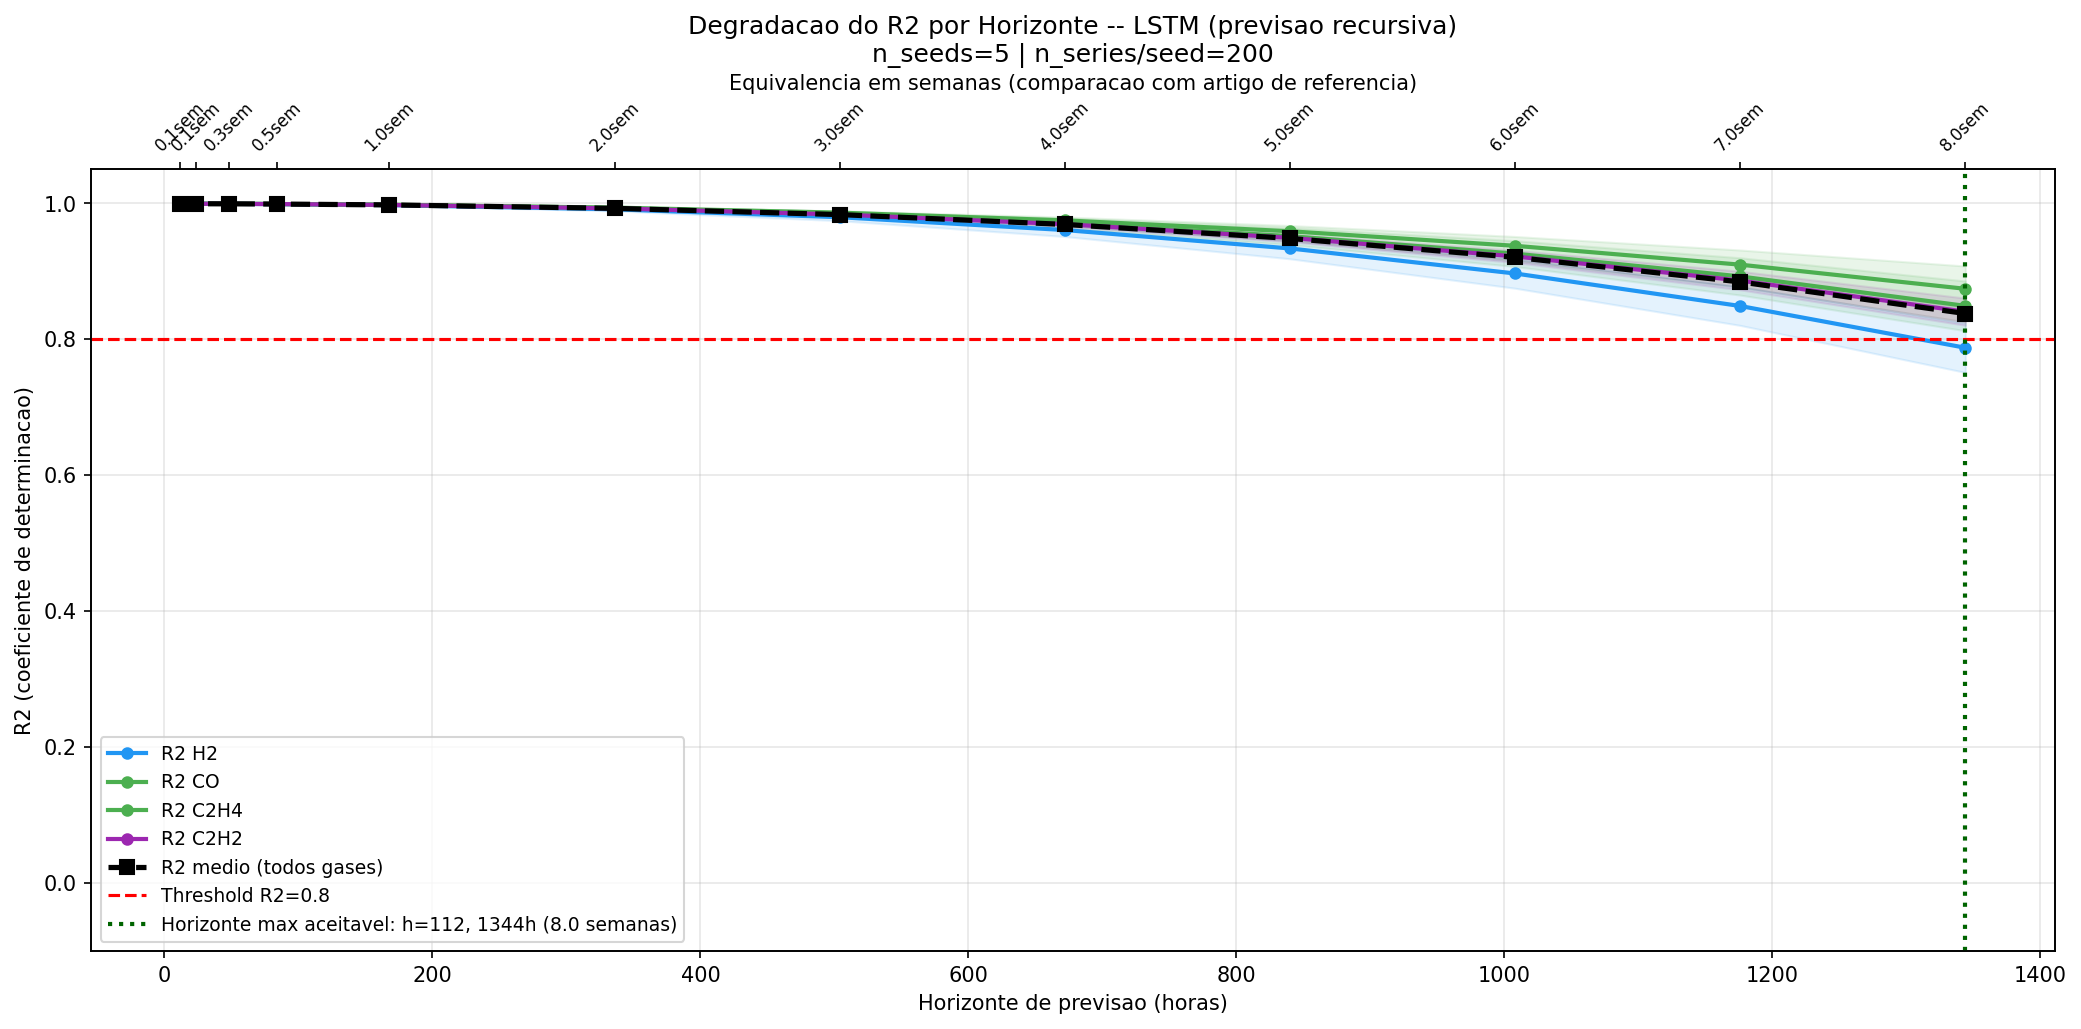
\includegraphics[width=0.85\textwidth]{figuras/lstm_multi_horizon_r2_norm.png}
\caption{Evolução do coeficiente de determinação ($R^2$) da LSTM em múltiplos horizontes temporais no conjunto de teste oficial.}
\label{fig:lstm_degradacao}
\fonte{Elaborado pelo autor.}
\end{figure}

A análise da evolução multi-horizonte mostra uma redução gradual da precisão preditiva, padrão esperado à medida que o horizonte temporal se estende. Até o horizonte de duas semanas ($h = 28$), o modelo mantém $R^2 \ge 0,9963$ com erro percentual médio de 2,33\%, nível adequado para acompanhamento em rotinas de manutenção. Mesmo no horizonte de sete semanas ($h = 98$), o $R^2$ médio situou-se em 0,8846, permanecendo acima do critério mínimo adotado. Com base nesse comportamento, escolheram-se as previsões de uma semana ($h = 14$) e duas semanas ($h = 28$) como atributos adicionais para os testes de classificação no Track A.

\section{Resultados do Track A: Desempenho e Avaliação da Hipótese Temporal}\label{sec:res_track_a}

O Track A avalia o diagnóstico em quatro classes de integridade operacional (Normal, Descarga Parcial -- PD, Descarga de Baixa Energia -- D1 e Falha Térmica de Baixa Temperatura -- T1) utilizando os dados de telemetria de \citeonline{katser2022}. O conjunto de teste contém 900 séries rotuladas: 731 casos normais, 38 de PD, 49 de D1 e 82 de T1. A hipótese investigada estabelecia que o fornecimento de concentrações futuras previstas pela LSTM enriqueceria os atributos de entrada do classificador XGBoost, gerando melhoria no diagnóstico pontual.

Para testar essa hipótese de forma controlada, compararam-se cinco configurações experimentais por meio de reamostragem por \textit{bootstrap} pareado e estratificado (5.000 iterações com reposição) sobre o conjunto de teste. A configuração C2 emprega o XGBoost com configuração fixa de referência sobre todos os 17 atributos (4 gases observados, 5 razões adaptadas e 8 previsões da LSTM para $h=14$ e $h=28$). A configuração C1 utiliza o Algoritmo Genético Melhorado (IGA) para selecionar variáveis e otimizar os hiperparâmetros sobre o mesmo espaço de 17 atributos. As configurações C5a e C5b avaliam o modelo puramente com os 9 atributos estáticos observados (sem dados da LSTM), sob parametrização de referência e otimizada por IGA, respectivamente. Por fim, a configuração C6 avalia o XGBoost treinado exclusivamente com as 8 previsões da LSTM. A Tabela~\ref{tab:track_a_ablacao} consolida os resultados obtidos.

\begin{table}[htbp]
\centering
\caption{Desempenho comparativo e teste de ablação da hipótese temporal no Track A (900 amostras de teste, 5 sementes).}
\label{tab:track_a_ablacao}
\resizebox{\textwidth}{!}{%
\begin{tabular}{lcccc}
\hline
\textbf{Configuração Avaliada} & \textbf{Atributos ($p$)} & \textbf{$F_1$-macro Teste} & \textbf{Desvio ($\sigma$)} & \textbf{IC 95\% Bootstrap} \\ \hline
C2: Ref. fixa com LSTM & 17 & 0,8911 & 0,0034 & $[0,8574; 0,9229]$ \\
C1: IGA com LSTM & 8 & 0,8909 & 0,0011 & $[0,8549; 0,9230]$ \\
C6: Ref. fixa apenas LSTM & 8 & 0,8888 & 0,0011 & $[0,8547; 0,9212]$ \\
C5a: Ref. fixa sem LSTM & 9 & 0,8855 & 0,0029 & $[0,8507; 0,9177]$ \\
C5b: IGA sem LSTM & 8 & 0,8796 & 0,0051 & $[0,8469; 0,9110]$ \\
C1 sem LSTM (pós-hoc) & 4 & 0,8280 & 0,0030 & $[0,7876; 0,8656]$ \\ \hline
\end{tabular}%
}
\fonte{Elaborado pelo autor.}
\end{table}

A pequena variação observada entre as sementes nas configurações de referência C2 ($\sigma = 0,0034$) e C5a ($\sigma = 0,0029$) decorre da subamostragem aleatória de instâncias (\texttt{subsample} = 0,90) adotada nessa parametrização. Ao comparar as configurações C2 e C5a para isolar o efeito da adição das previsões da LSTM com hiperparâmetros fixos, verifica-se (Tabela~\ref{tab:track_a_pareada}) que a diferença pontual foi de $\Delta F_1 = +0,0056$ ($+0,56\%$), com intervalo de confiança de 95\% entre $-0,0037$ e $+0,0150$, e valor de $p \approx 0,2384$. Como o intervalo de confiança engloba o valor zero ($p > 0,05$), conclui-se que a inclusão das projeções futuras da LSTM não trouxe ganho estatisticamente significativo para o diagnóstico pontual.

\begin{table}[htbp]
\centering
\caption{Comparações pareadas via bootstrap (5.000 iterações) no Track A.}
\label{tab:track_a_pareada}
\resizebox{\textwidth}{!}{%
\begin{tabular}{lcccc}
\hline
\textbf{Contraste Pareado} & \textbf{$\Delta F_1$ Pontual} & \textbf{IC 95\% Bootstrap} & \textbf{Valor $p$} & \textbf{Significância} \\ \hline
C2 vs. C5a (efeito LSTM na ref. fixa) & $+0,0056$ & $[-0,0037; +0,0150]$ & 0,2384 & Não significativa \\
C2 vs. C6 (todos vs. apenas LSTM) & $+0,0023$ & $[-0,0081; +0,0131]$ & 0,6604 & Não significativa \\
C1 vs. C2 (IGA vs. ref. fixa completa) & $-0,0003$ & $[-0,0137; +0,0124]$ & 0,9956 & Não significativa \\
C1 vs. C5b (efeito LSTM sob IGA) & $+0,0112$ & $[-0,0103; +0,0339]$ & 0,3308 & Não significativa \\
C5b vs. C5a (IGA vs. ref. fixa sem LSTM) & $-0,0059$ & $[-0,0247; +0,0118]$ & 0,5412 & Não significativa \\ \hline
\end{tabular}%
}
\fonte{Elaborado pelo autor.}
\end{table}

A razão física e matemática para a ausência de ganho adicional reside na forte correlação entre as leituras observadas no momento atual e as projeções estimadas pela rede neural. No conjunto de treino, o coeficiente de correlação de Pearson ($r$) entre o valor observado e a projeção futura foi de 0,9993 e 0,9974 para o $\text{H}_2$ nos horizontes de 14 e 28 passos, 0,9997 e 0,9990 para o $\text{CO}$, 0,9994 e 0,9981 para o $\text{C}_2\text{H}_4$, e 0,9995 e 0,9985 para o $\text{C}_2\text{H}_2$. Em todas as séries, $r^2$ superou 0,994. Isso mostra que, em transformadores com taxas graduais de degradação, as medições do instante presente já contêm quase toda a informação necessária para a classificação, de modo que a projeção futura atua na prática como uma variável fortemente redundante em relação à leitura atual.

Por outro lado, o Algoritmo Genético Melhorado (IGA) demonstrou grande utilidade na simplificação do modelo. A comparação entre C1 e C2 resultou em diferença mínima ($\Delta F_1 = -0,0003$ e $p \approx 0,9956$), demonstrando desempenho equivalente. Contudo, enquanto o modelo C2 utiliza 17 variáveis, o algoritmo genético selecionou um subconjunto enxuto de apenas 8 variáveis: $\text{CO}_{\text{obs}}$, $\text{H}_2/\text{C}_2\text{H}_2$, $\text{C}_2\text{H}_2/\text{TH}_{\text{katser}}$, $\text{C}_2\text{H}_4/\text{TH}_{\text{katser}}$, $\text{H}_{2,\text{h14}}$, $\text{H}_{2,\text{h28}}$, $\text{C}_2\text{H}_{4,\text{h28}}$ e $\text{C}_2\text{H}_{2,\text{h28}}$. Como ilustrado na Figura~\ref{fig:tradeoff_complexidade}, obteve-se uma redução de 53\% no número de atributos sem perda de desempenho diagnóstico, o que simplifica o processamento e facilita a implantação prática em sistemas industriais.

\begin{figure}[htbp]
\centering
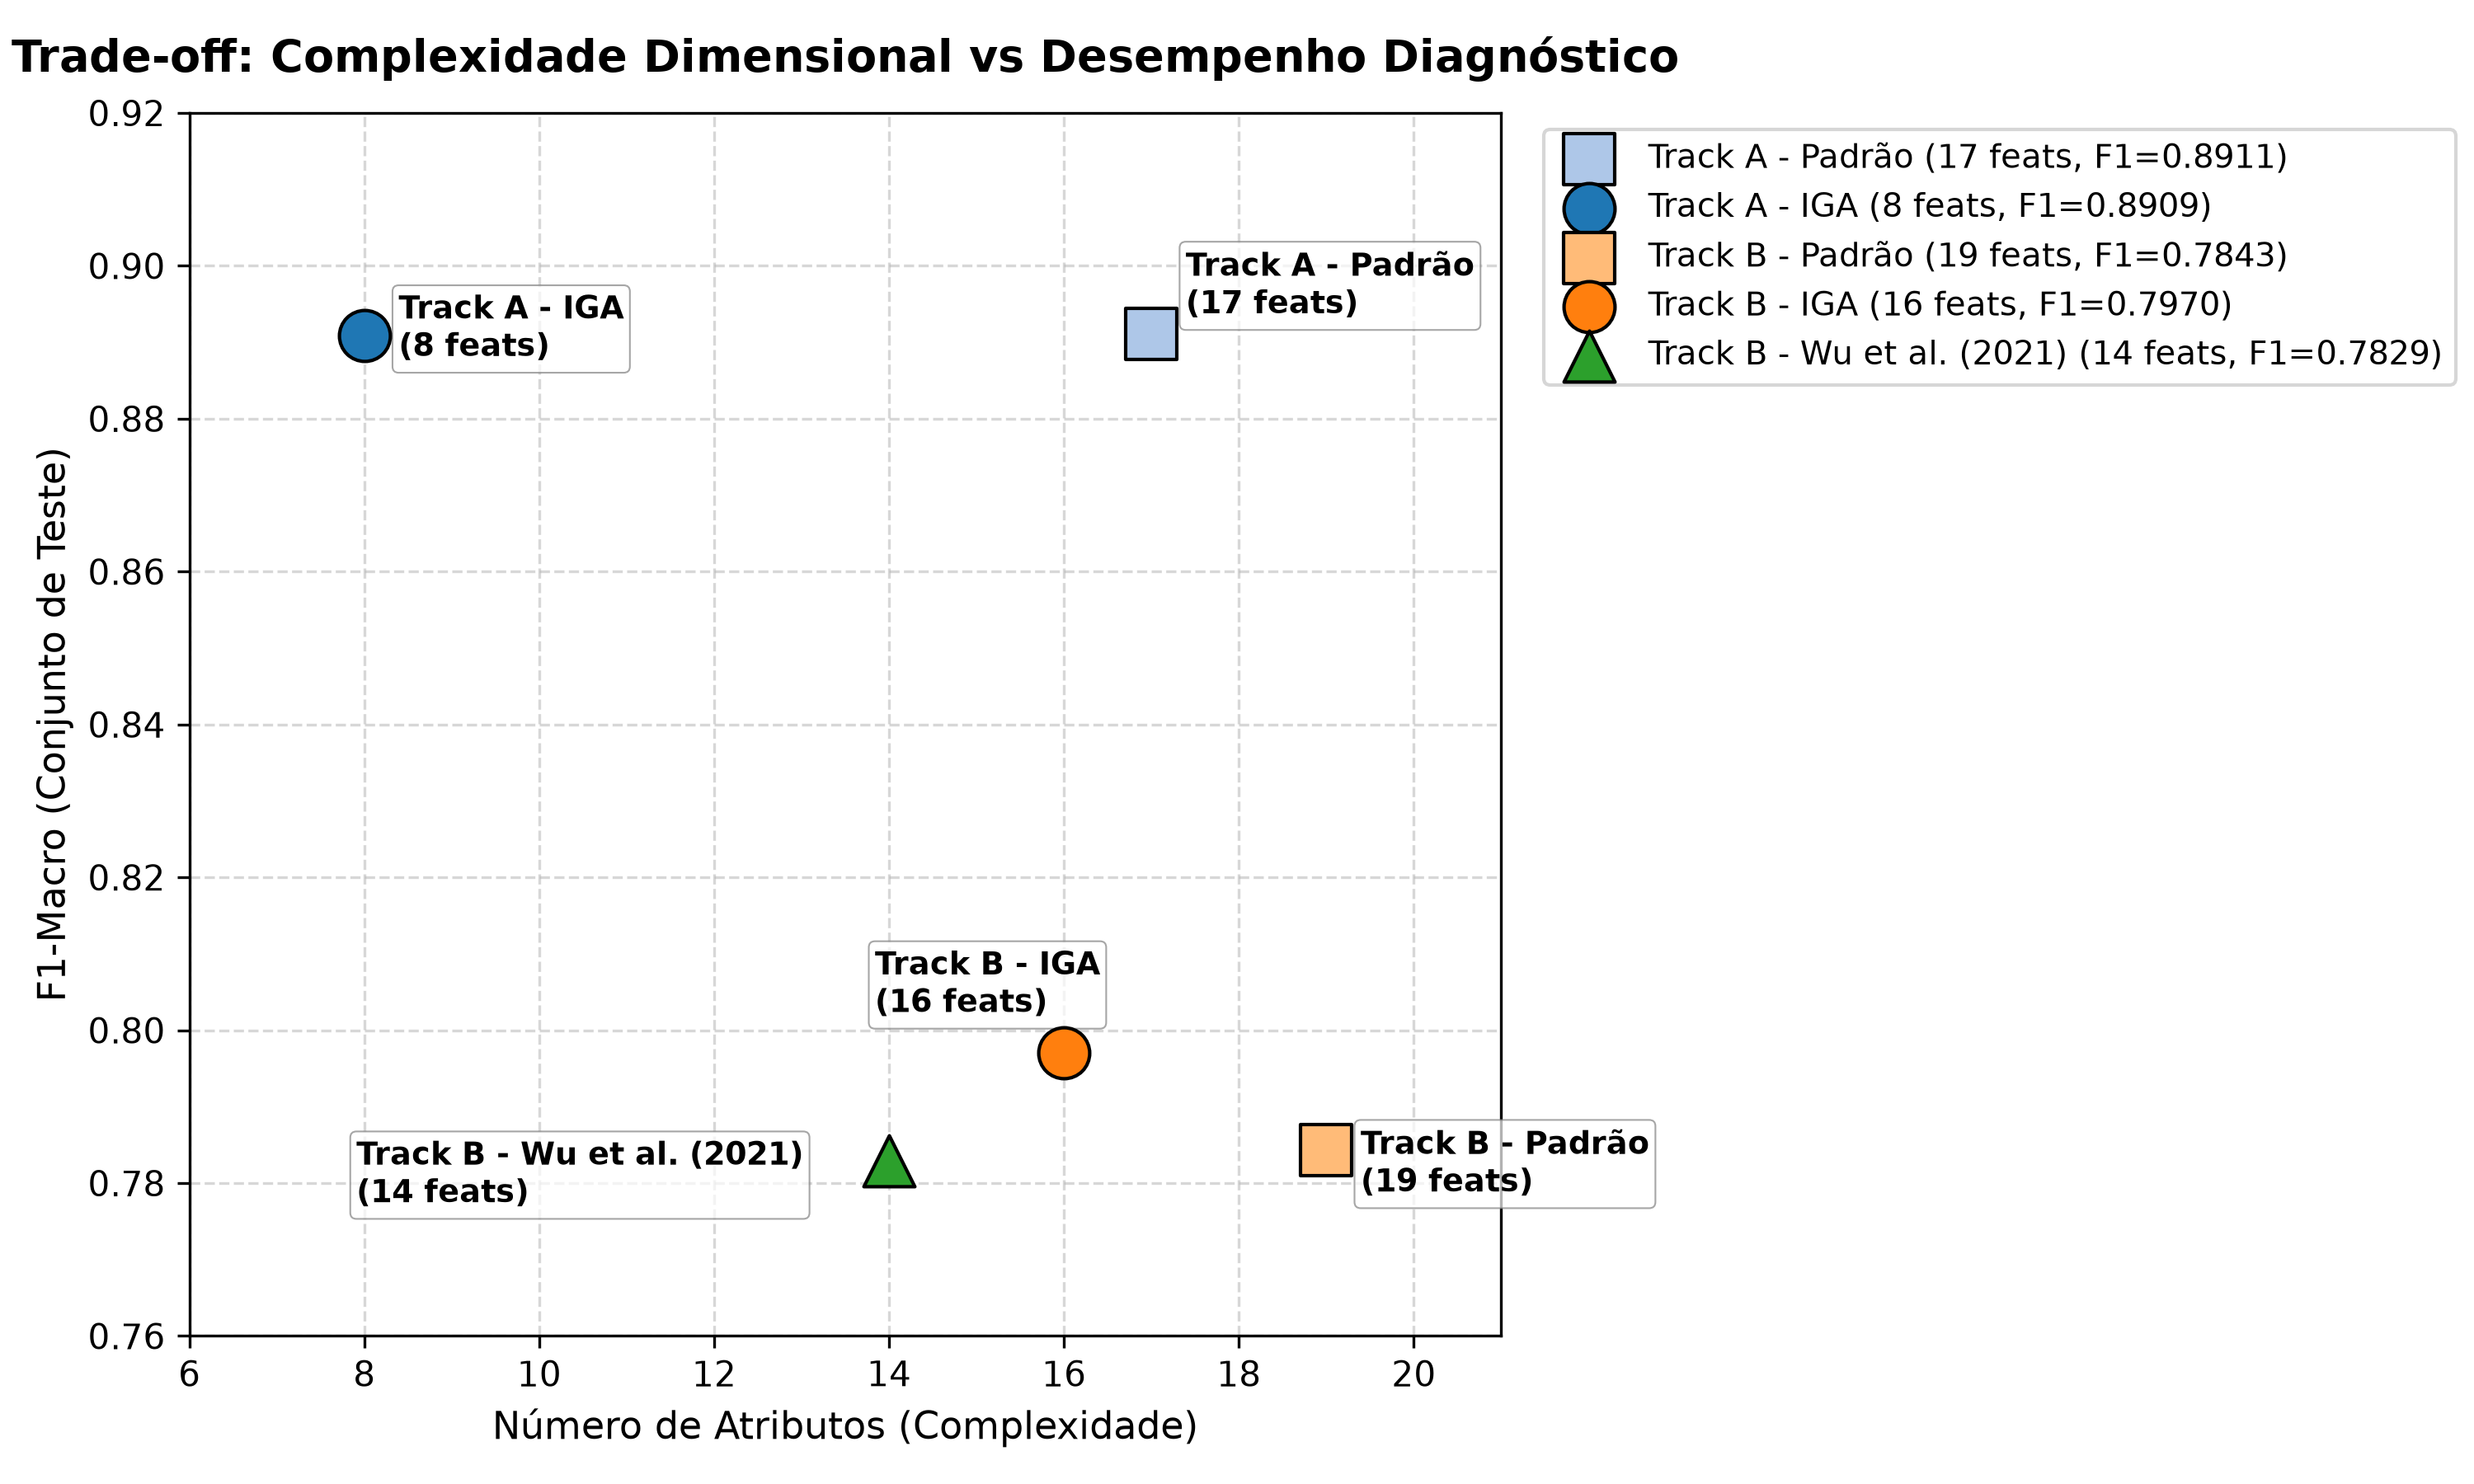
\includegraphics[width=0.85\textwidth]{figuras/xgb_tradeoff_complexity.png}
\caption{Relação entre complexidade dimensional e desempenho diagnóstico no Track A.}
\label{fig:tradeoff_complexidade}
\fonte{Elaborado pelo autor.}
\end{figure}

\begin{figure}[htbp]
\centering
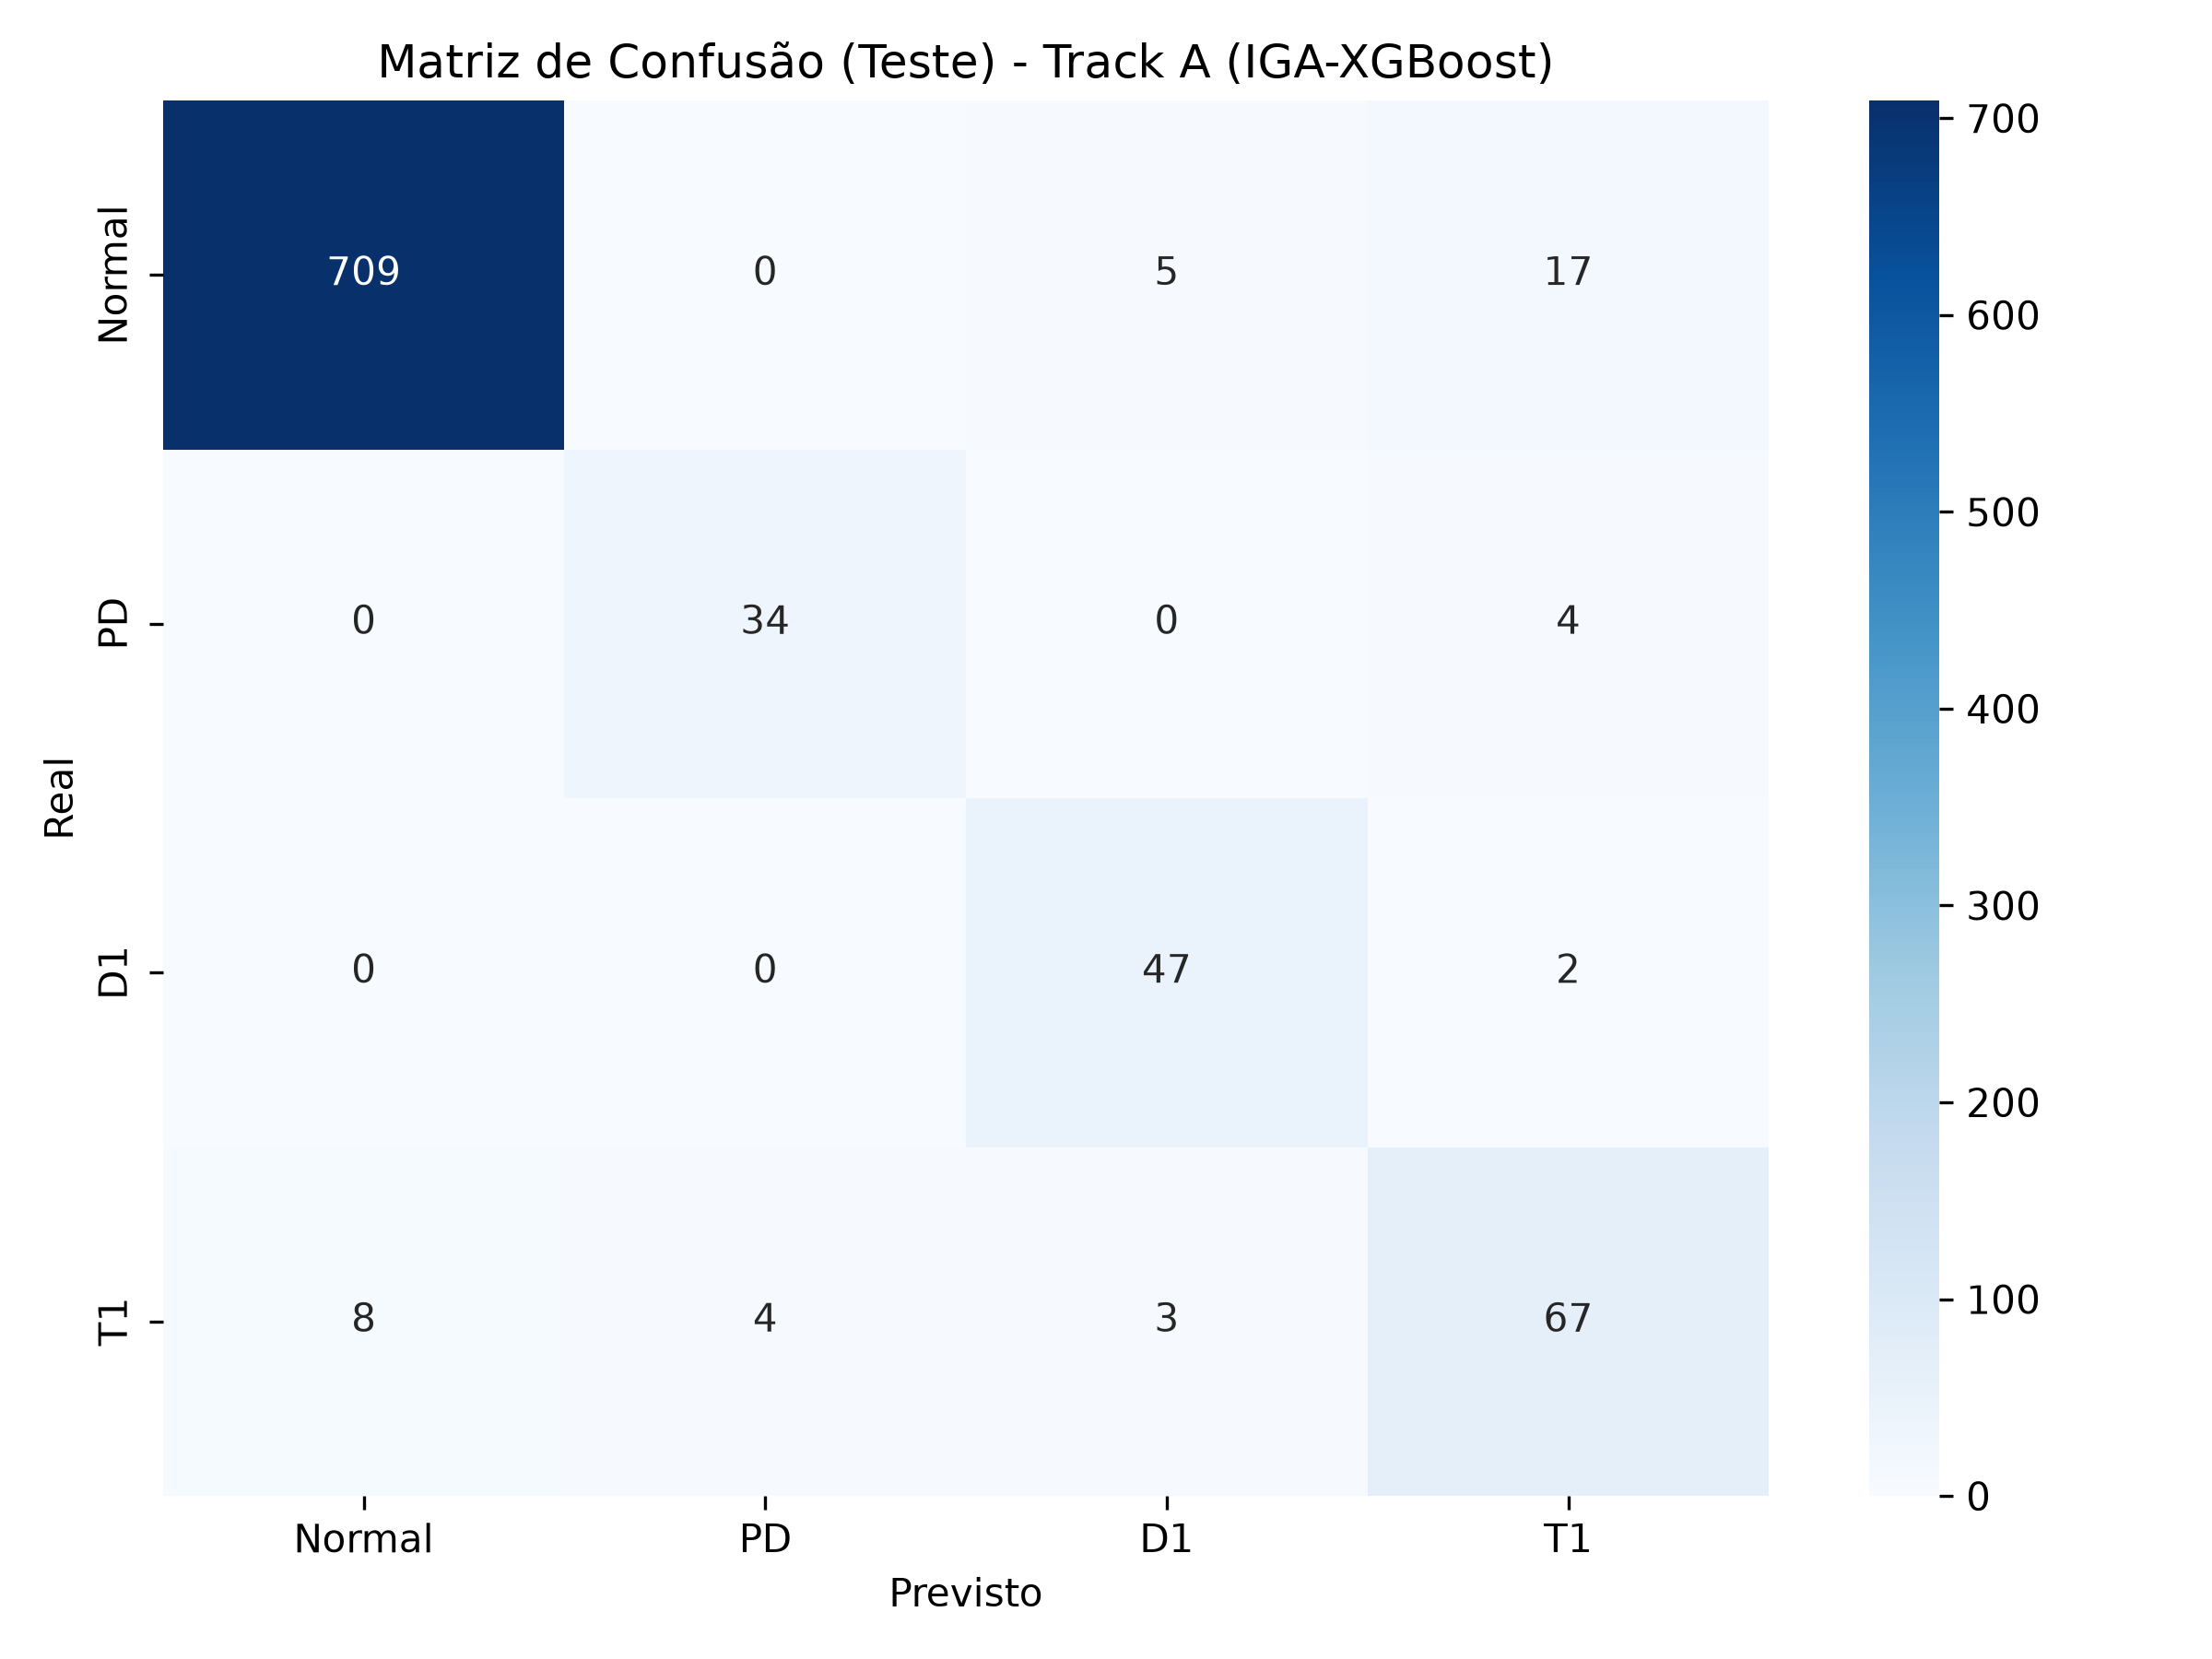
\includegraphics[width=0.85\textwidth]{figuras/xgb_confusion_track_a.png}
\caption{Matriz de confusão das predições diagnósticas para o Track A no conjunto de teste oficial.}
\label{fig:matriz_track_a}
\fonte{Elaborado pelo autor.}
\end{figure}

A matriz de confusão apresentada na Figura~\ref{fig:matriz_track_a} mostra boa capacidade de acerto nas classes avaliadas: 709 acertos em 731 amostras na condição Normal (recall de 97,0\% e $F_1 = 0,979$), 34 acertos em 38 amostras em Descargas Parciais (PD, com recall de 89,5\% e $F_1 = 0,895$) e 47 acertos em 49 amostras em Descargas de Baixa Energia (D1, com recall de 95,9\% e $F_1 = 0,904$). Na classe de falhas térmicas incipientes T1, registraram-se 67 acertos em 82 casos (recall de 81,7\% e $F_1 = 0,779$). As principais confusões ocorreram entre a condição Normal e a classe T1 (17 amostras normais classificadas como T1 e 8 amostras de T1 classificadas como normais). Esse padrão é condizente com a física do problema: sobreaquecimentos térmicos leves em temperaturas inferiores a 300~$^\circ\text{C}$ geram pequenas quantidades de gás, que se misturam facilmente com as concentrações residuais do envelhecimento natural do óleo isolante.

\section{Resultados do Track B: Diagnóstico Multiclasse e Limites dos Dados}\label{sec:res_track_b}

O Track B avalia a classificação entre os sete estados operacionais da norma IEC 60599 (Normal, PD, D1, D2, T1, T2 e T3) a partir da base estática consolidada de 1.962 amostras únicas, após o procedimento de saneamento e remoção das 359 amostras redundantes ou conflitantes. O conjunto de teste contém 295 amostras: 106 normais, 17 de PD, 41 de D1, 33 de D2, 16 de T1, 16 de T2 e 66 de T3. O objetivo foi analisar o desempenho de modelos baseados em árvores em comparação com os métodos normativos e com a formulação de referência de \citeonline{wu2021}.

Avaliaram-se cinco abordagens: o modelo IGA-XGBoost deste estudo (C3), o XGBoost com configuração fixa de referência sobre os 19 atributos candidatos (C4), a adaptação do espaço de 18 atributos candidatos de \citeonline{wu2021} com 14 variáveis selecionadas pelo IGA (M3), o Triângulo 1 de Duval (M2) e o Método das Razões da norma IEC 60599 (M1). A Tabela~\ref{tab:track_b_desempenho} apresenta as métricas obtidas no conjunto de teste e o resultado consolidado em validação cruzada repetida em 5 repetições com 5 dobras (Repeated Stratified $5 \times 5$ CV, totalizando 25 dobras de teste).

\begin{table}[htbp]
\centering
\caption{Desempenho diagnóstico multiclasse no Track B sobre sete categorias operacionais.}
\label{tab:track_b_desempenho}
\resizebox{\textwidth}{!}{%
\begin{tabular}{lccccc}
\hline
\textbf{Modelo / Método} & \textbf{Atributos} & \textbf{$F_1$-macro Teste} & \textbf{IC 95\% Teste} & \textbf{$F_1$-macro CV $5\times 5$} & \textbf{IC 95\% CV} \\ \hline
C3: IGA-XGBoost & 16 & 0,7970 & $[0,7392; 0,8515]$ & 0,7516 & $[0,7406; 0,7626]$ \\
C4: XGBoost Ref. Fixa & 19 & 0,7843 & $[0,7259; 0,8376]$ & 0,7616 & $[0,7527; 0,7705]$ \\
M3: Wu et al. (2021) & 14 & 0,7829 & $[0,7261; 0,8376]$ & 0,7654 & $[0,7555; 0,7752]$ \\
M2: Triângulo de Duval & 3 gases & 0,3634 & $[0,3101; 0,4135]$ & -- & -- \\
M1: Razões IEC 60599 & 5 gases & 0,2569 & $[0,1944; 0,3143]$ & -- & -- \\ \hline
Linha de base (5 gases) & 5 & 0,7250 & $[0,6587; 0,7851]$ & 0,7082 & $[0,6965; 0,7200]$ \\ \hline
\end{tabular}%
}
\fonte{Elaborado pelo autor.}
\end{table}

A comparação pareada por \textit{bootstrap} no conjunto de teste mostrou que a diferença entre o modelo C3 e o modelo adaptado de Wu et al. (M3) foi de $\Delta F_1 = +0,0141$, com intervalo de confiança $[-0,0054; +0,0368]$ e $p \approx 0,1824$. Do mesmo modo, o contraste entre C3 e o XGBoost de referência C4 resultou em $\Delta F_1 = +0,0127$ com intervalo $[-0,0211; +0,0490]$ e $p \approx 0,4680$. Em ambos os casos, a nulidade está contida no intervalo de confiança, indicando equivalência estatística entre os modelos baseados em gradiente de árvores. Esse resultado é reforçado pela validação cruzada repetida em 25 dobras, na qual os intervalos de C3 ($0,7516 \pm 0,0281$), C4 ($0,7616 \pm 0,0226$) e M3 ($0,7654 \pm 0,0252$) apresentam sobreposição quase completa (em que $\pm$ indica o desvio-padrão entre as 25 dobras).

Do ponto de vista prático e estatístico, essa estabilidade de resultados em torno de 76\% a 78\% de $F_1$-macro aponta para um limite prático nos dados de DGA estáticos baseados exclusivamente em cinco gases. Como todas as variáveis derivadas (razões e percentuais) são obtidas a partir das mesmas cinco concentrações primárias ($\text{H}_2$, $\text{CH}_4$, $\text{C}_2\text{H}_6$, $\text{C}_2\text{H}_4$ e $\text{C}_2\text{H}_2$), a engenharia de atributos não adiciona informação externa nova. Ela auxilia o classificador ao explicitar relações físico-químicas conhecidas (superando o modelo treinado apenas com gases brutos, que obteve $F_1 \approx 0,7082$), mas não elimina a sobreposição física entre falhas que geram perfis de gases muito semelhantes. Note-se ainda que o conjunto de 18 atributos candidatos de Wu et al. difere do espaço de C3 unicamente pela omissão da razão $\text{C}_2\text{H}_2/\text{CH}_4$, o que justifica a proximidade estreita de comportamento entre M3 e C3.

\begin{figure}[htbp]
\centering
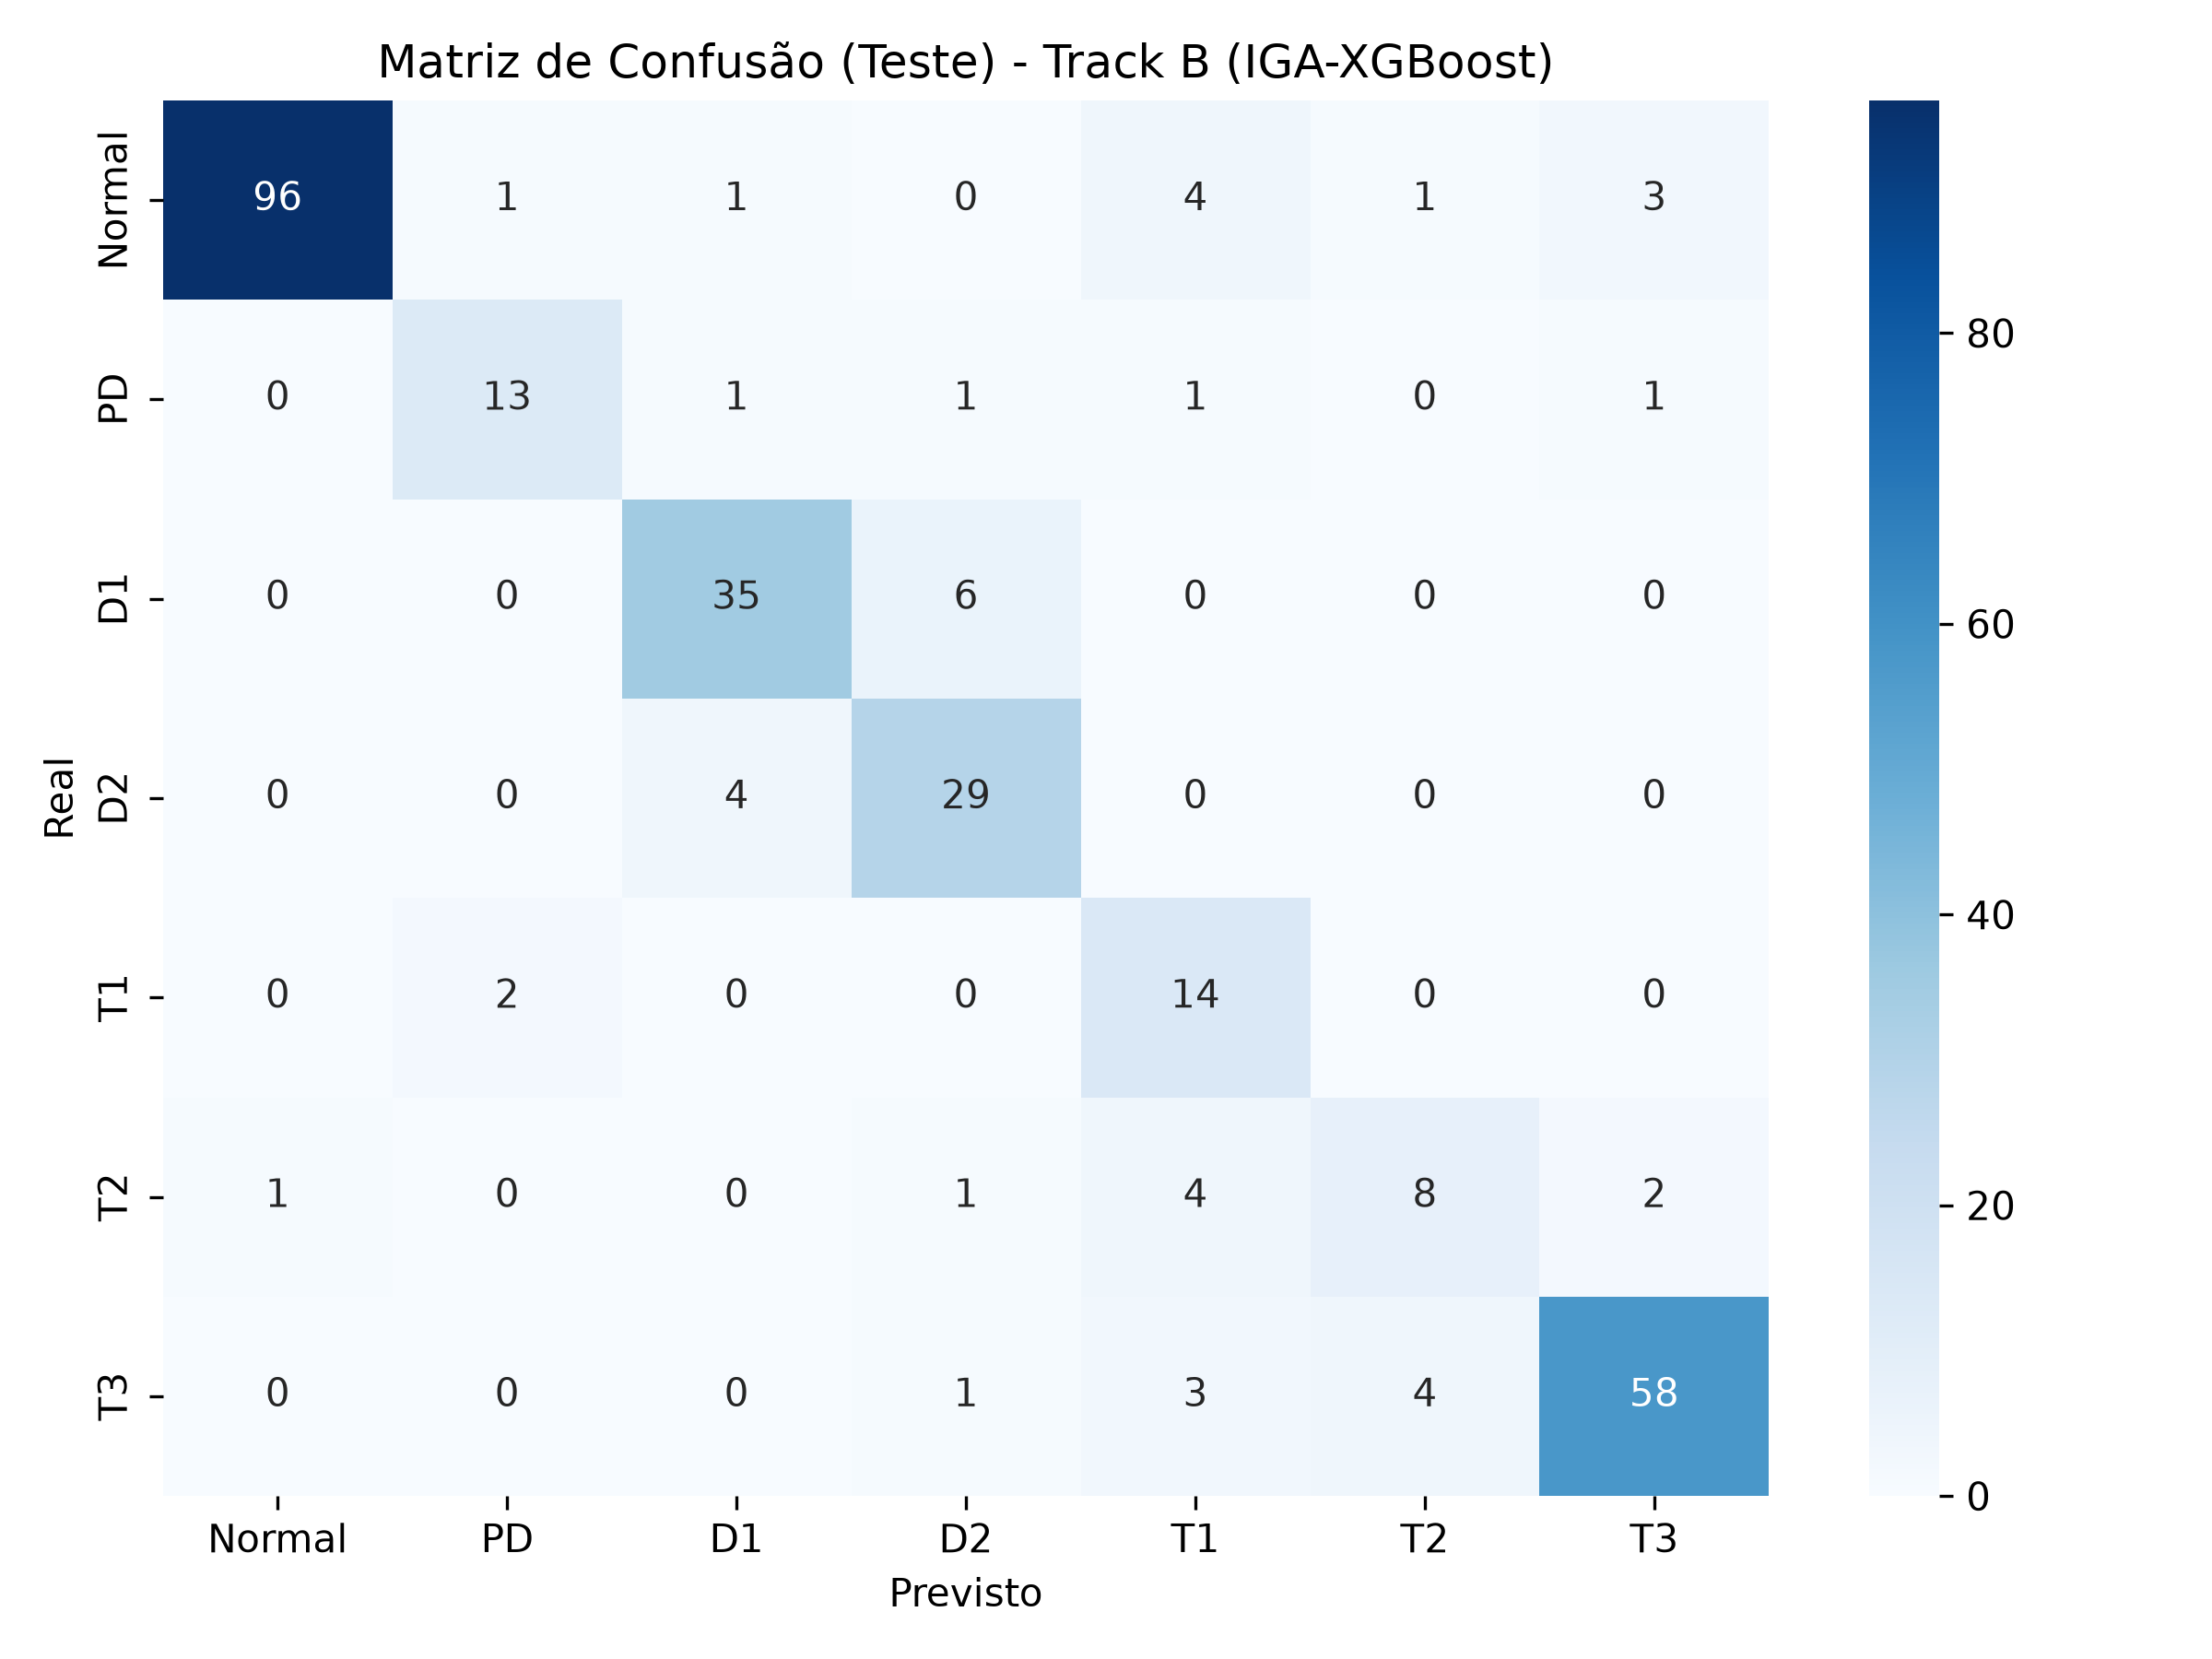
\includegraphics[width=0.85\textwidth]{figuras/xgb_confusion_track_b.png}
\caption{Matriz de confusão do modelo C3 (IGA-XGBoost) no teste de sete classes do Track B.}
\label{fig:matriz_track_b}
\fonte{Elaborado pelo autor.}
\end{figure}

A matriz de confusão do modelo C3 (Figura~\ref{fig:matriz_track_b}) ilustra os principais pontos de confusão no Track B. Observam-se 10 erros entre descargas de baixa energia (D1) e alta energia (D2): 6 amostras de D1 previstas como D2 e 4 amostras de D2 previstas como D1. Essa troca reflete uma transição contínua entre centelhamentos intermitentes e arcos elétricos mais intensos, onde a proporção de acetileno e etileno pode variar sutilmente. Além disso, as classes térmicas incipientes T1 e T2 registraram acertos mais modestos ($F_1 = 0,667$ em T1 com 14 acertos em 16 casos, e $F_1 = 0,552$ em T2 com 8 acertos em 16 casos), refletindo tanto a menor quantidade de amostras dessas classes na base quanto a proximidade das faixas térmicas de degradação do óleo. Em contrapartida, as classes Normal e T3 sustentaram desempenhos elevados, com índices superiores a 0,90.

\section{Auditoria Normativa: Divergência dos Métodos Tradicionais}\label{sec:res_auditoria}

Os índices de desempenho obtidos pelos métodos normativos tradicionais na Tabela~\ref{tab:track_b_desempenho} ($F_1 = 0,3634$ para o Triângulo 1 de Duval e $F_1 = 0,2569$ para a IEC 60599) são sensivelmente inferiores às taxas comumente citadas na literatura técnica, frequentemente reportadas entre 70\% e 90\%. Essa diferença motivou uma verificação cuidadosa tanto da implementação dos algoritmos quanto das características dos dados de campo.

Para verificar a conformidade dos algoritmos normativos implementados, as regras de classificação foram confrontadas analiticamente com os parâmetros da norma IEC 60599 e com a partição geométrica do Triângulo 1 de Duval. A rotina do Triângulo 1 reproduziu as regiões canônicas centrais, sendo que variações pontuais em casos de teste decorrem de fronteiras limítrofes entre zonas vizinhas (como a transição entre T1 e T2 em $\% \text{C}_2\text{H}_4 \approx 20\%$) e da zona mista DT. Do mesmo modo, a rotina das Razões da IEC 60599 foi confrontada diretamente com os intervalos tabulares da norma, confirmando a correspondência lógica dos critérios de decisão.

A auditoria sobre a base consolidada de 1.962 amostras, resumida na Tabela~\ref{tab:auditoria_normativa}, evidenciou duas razões principais para a divergência observada.

\begin{table}[htbp]
\centering
\caption{Concordância entre os rótulos da base e os diagnósticos da IEC 60599 e do Triângulo de Duval.}
\label{tab:auditoria_normativa}
\resizebox{\textwidth}{!}{%
\begin{tabular}{lcccccc}
\hline
\textbf{Classe} & \textbf{Total} & \multicolumn{2}{c}{\textbf{IEC 60599}} & \multicolumn{3}{c}{\textbf{Triângulo 1 de Duval}} \\ \cline{3-4} \cline{5-7}
\textbf{Rotulada} & \textbf{($N$)} & \textbf{Concordância} & \textbf{Não Determinado} & \textbf{Concordância} & \textbf{Zona DT} & \textbf{Principal Desvio} \\ \hline
Normal & 707 & 0,0\% & 14,0\% & 0,0\% & 0,7\% & 89,0\% predito como T1 \\
PD & 111 & 14,4\% & 80,2\% & 14,4\% & 4,5\% & 52,3\% predito como T1 \\
D1 & 273 & 24,2\% & 71,4\% & 76,2\% & 4,8\% & 14,7\% predito como D2 \\
D2 & 221 & 15,8\% & 40,7\% & 58,4\% & 10,0\% & 24,4\% predito como D1 \\
T1 & 107 & 48,6\% & 36,4\% & 31,8\% & 2,8\% & 41,1\% predito como T2 \\
T2 & 108 & 64,8\% & 17,6\% & 38,9\% & 10,2\% & 39,8\% predito como T3 \\
T3 & 435 & 31,3\% & 14,0\% & 38,4\% & 8,5\% & 39,1\% predito como T2 \\ \hline
\end{tabular}%
}
\fonte{Elaborado pelo autor.}
\end{table}

A primeira causa decorre do próprio escopo das normas: tanto o Triângulo de Duval quanto as razões da IEC foram projetados para determinar o tipo de defeito em transformadores que já apresentaram gases totais acima dos limites normais de atenção. Por essa razão, esses métodos não possuem uma classe para o estado Normal em suas tabelas e regiões. Quando aplicados a uma base completa que contém equipamentos saudáveis, o Triângulo de Duval classifica 89,0\% das amostras normais como falha térmica T1, e a IEC 60599 classifica 83,6\% como T1, zerando a precisão nessa classe (que é a mais numerosa). Além disso, a IEC 60599 resulta em elevados índices de diagnóstico Não Determinado nas descargas (80,2\% em PD e 71,4\% em D1, além de 36,4\% em T1 e 40,7\% em D2), gerando laudos inconclusivos para grande parte dos registros práticos.

A segunda causa envolve uma divergência nas características das amostras rotuladas como T3 na base compilada. Pelos critérios clássicos da IEC 60599, uma falha térmica severa ($T > 700\ ^\circ\text{C}$) provoca intensa quebra de etano em etileno, exigindo razão $\text{C}_2\text{H}_4/\text{C}_2\text{H}_6 > 4$. Contudo, na base analisada, a mediana dessa razão para os casos anotados como T3 foi de apenas 0,25. Por essa razão, os métodos normativos acabam classificando grande parte desses casos como sobreaquecimentos moderados (T1 ou T2). O XGBoost reproduz os rótulos desta base com maior taxa de acerto do que os métodos normativos, embora isso reflita o ajuste supervisionado à distribuição anotada e não garanta, por si só, que todos os laudos originais estejam fisicamente corretos.

\section{Interpretabilidade Físico-Química via SHAP}\label{sec:res_shap}

Para que modelos de aprendizado de máquina sejam adotados com segurança em sistemas elétricos de potência, é fundamental compreender a coerência física das decisões. Para analisar essa relação, aplicou-se o algoritmo TreeSHAP \cite{lundberg2020} ao modelo XGBoost. As contribuições parciais ($\phi_i$) foram calculadas diretamente no espaço aditivo de margens lineares (\textit{log-odds}) de cada classe, garantindo que a soma dos valores de Shapley somada ao valor médio basal reproduza a pontuação contínua do modelo antes da softmax ($\sum_{i=1}^{M} \phi_i + \phi_0 = f(x)$).

\subsection{Estabilidade do Ranking Global}

Antes de analisar as regras aprendidas, avaliou-se a estabilidade do ordenamento de importância em relação a variações aleatórias de treinamento. Para cada uma das cinco sementes do modelo C3 no Track B, calculou-se o vetor de importância global média absoluta ($E[|\phi_i|]$). A correlação de postos de Spearman ($\rho$) entre os rankings das cinco sementes alcançou média de $\rho = 0,9541$. O alto valor de correlação confirma que o modelo aprendeu critérios consistentes a partir dos dados, e não padrões instáveis decorrentes da amostragem.

\subsection{Relevância por Classe e Agrupamento por Famílias Químicas}

Para contornar a dificuldade de interpretação gerada pela correlação entre variáveis derivadas do mesmo gás, somou-se a contribuição dos atributos em quatro grupos químicos: derivados de acetileno ($\text{C}_2\text{H}_2$), derivados de etileno ($\text{C}_2\text{H}_4$), derivados de metano ($\text{CH}_4$) e gases brutos. Pela aditividade do TreeSHAP, a soma dos valores de $\phi$ dentro de cada grupo reflete o peso total daquela família na decisão. A Figura~\ref{fig:shap_heatmap} apresenta o mapa de calor com a importância de cada variável por classe, e a Figura~\ref{fig:shap_grouped} resume as importâncias agrupadas pelas quatro famílias de gases.

\begin{figure}[htbp]
\centering
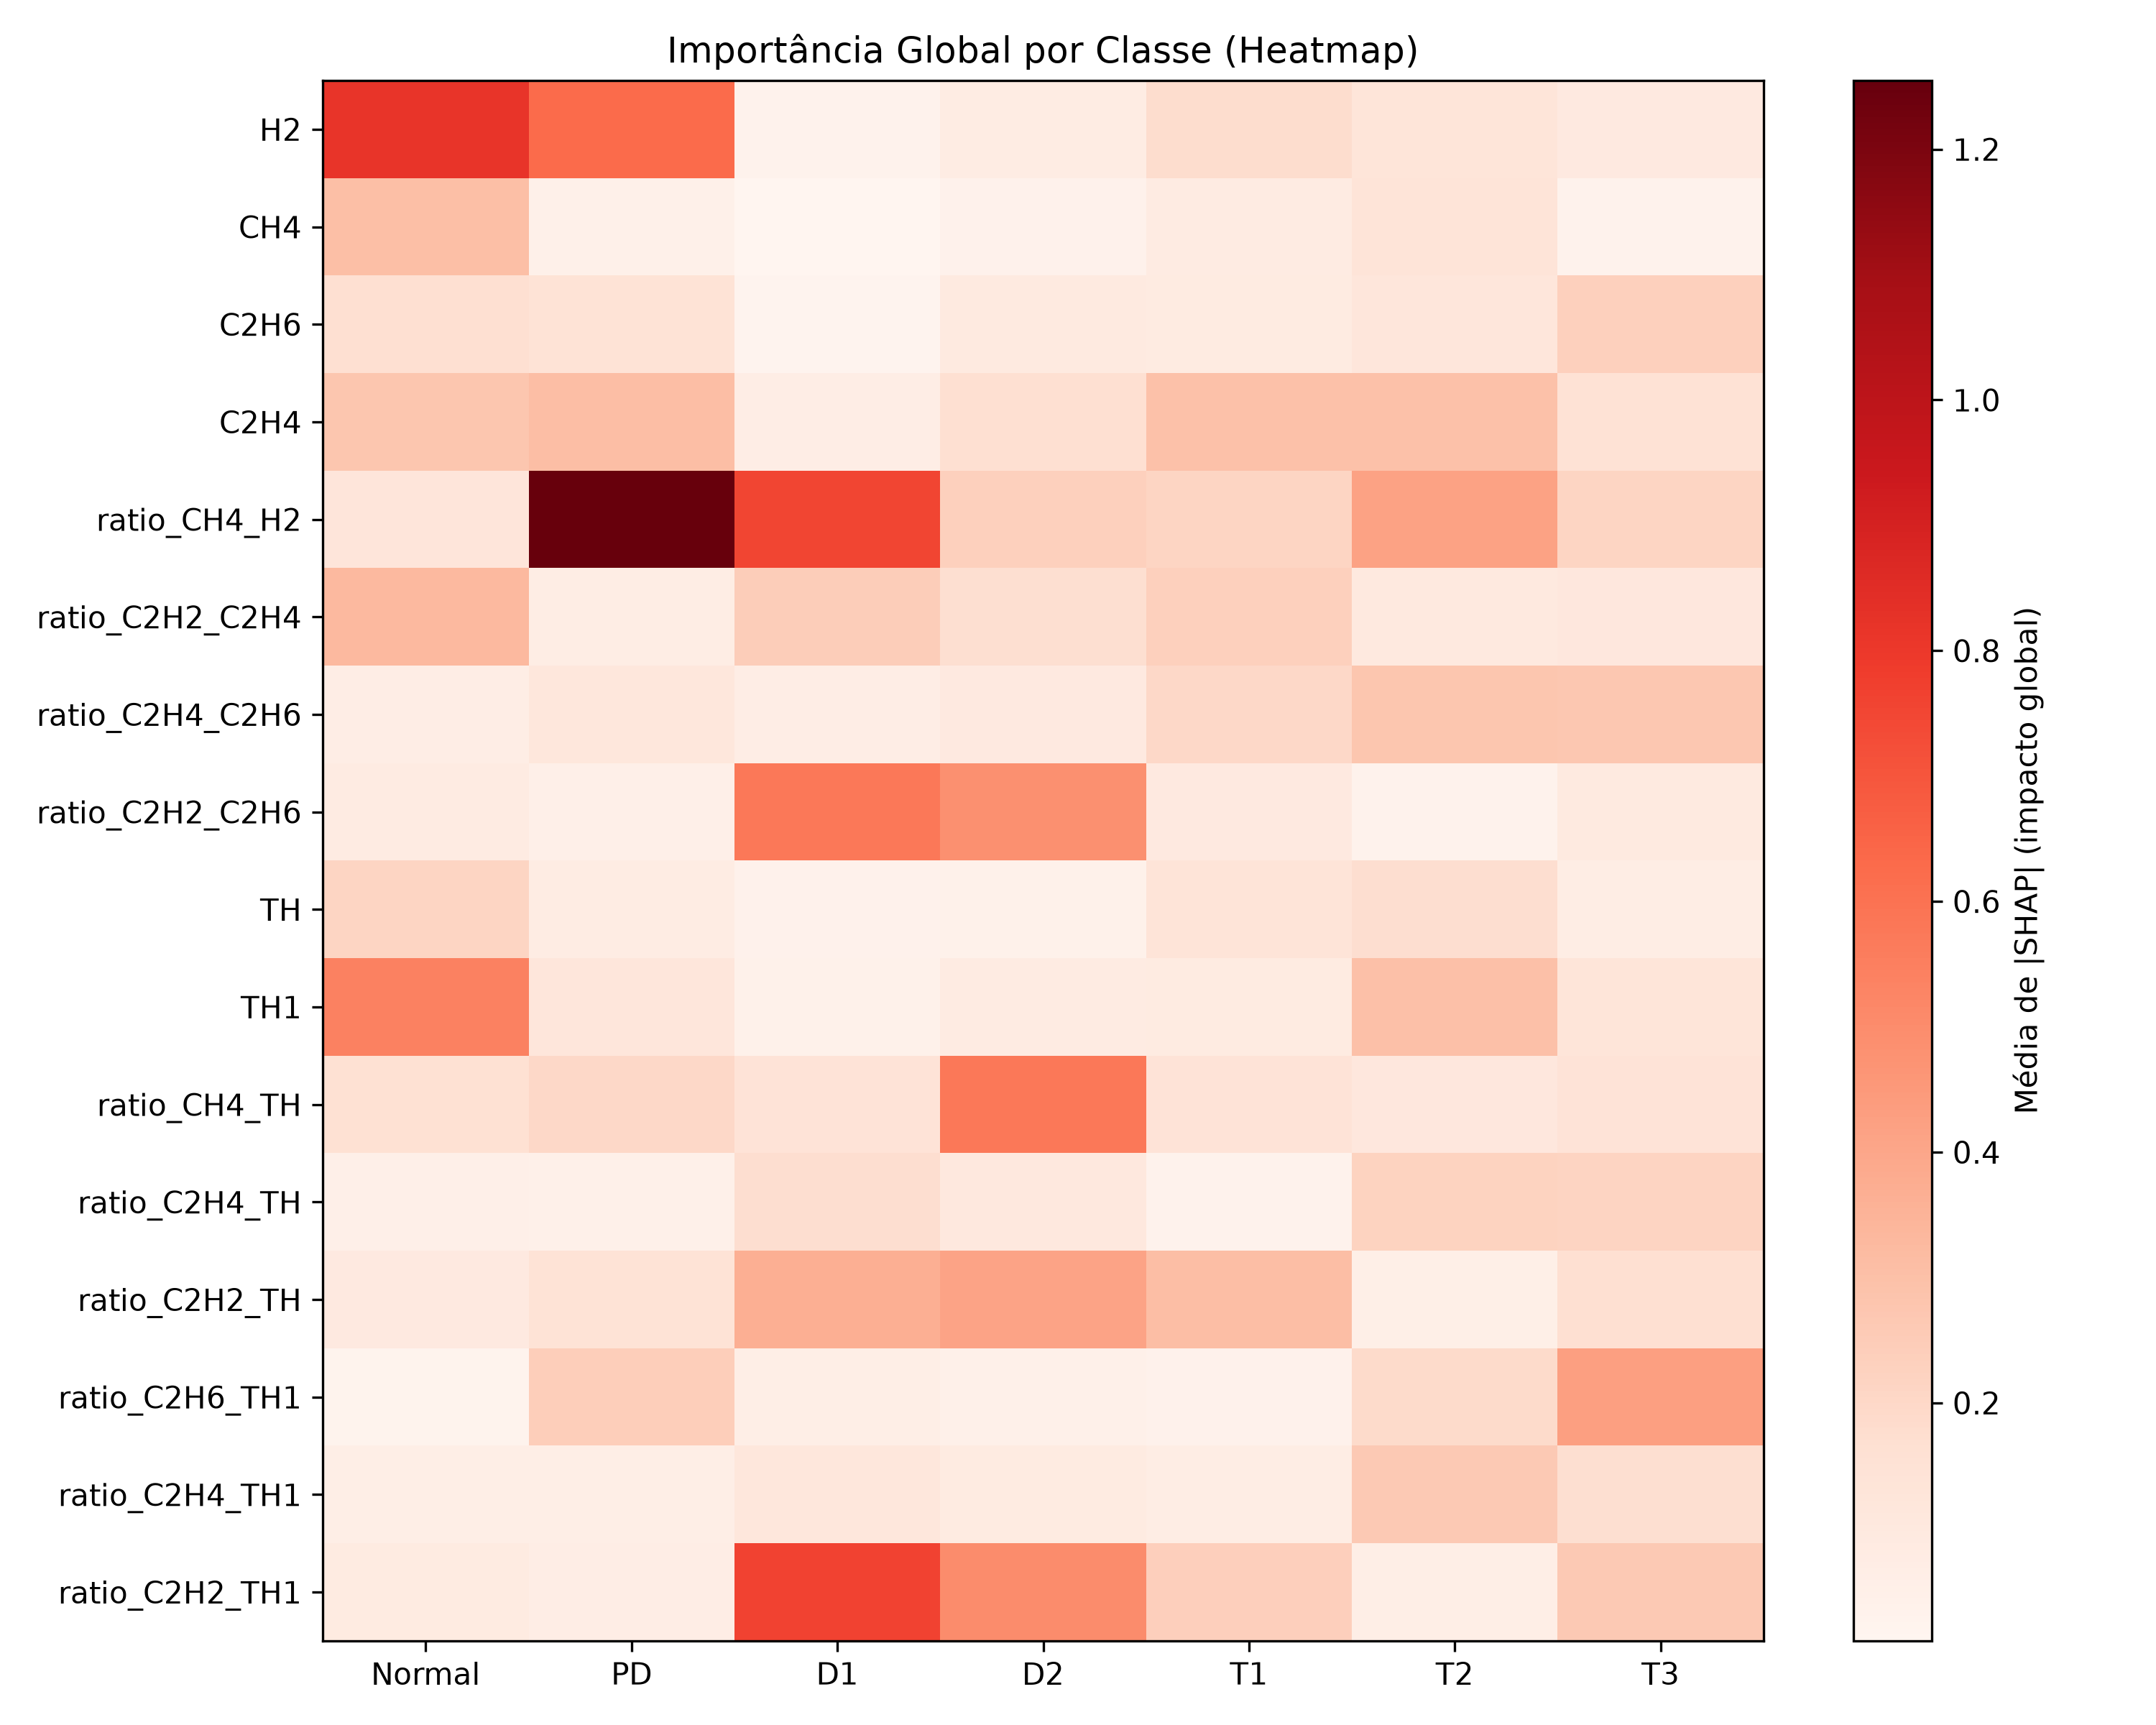
\includegraphics[width=0.85\textwidth]{figuras/fase6/fig1_heatmap_track_b.png}
\caption{Mapa de calor da importância média absoluta do SHAP por classe operacional no Track B.}
\label{fig:shap_heatmap}
\fonte{Elaborado pelo autor.}
\end{figure}

\begin{figure}[htbp]
\centering
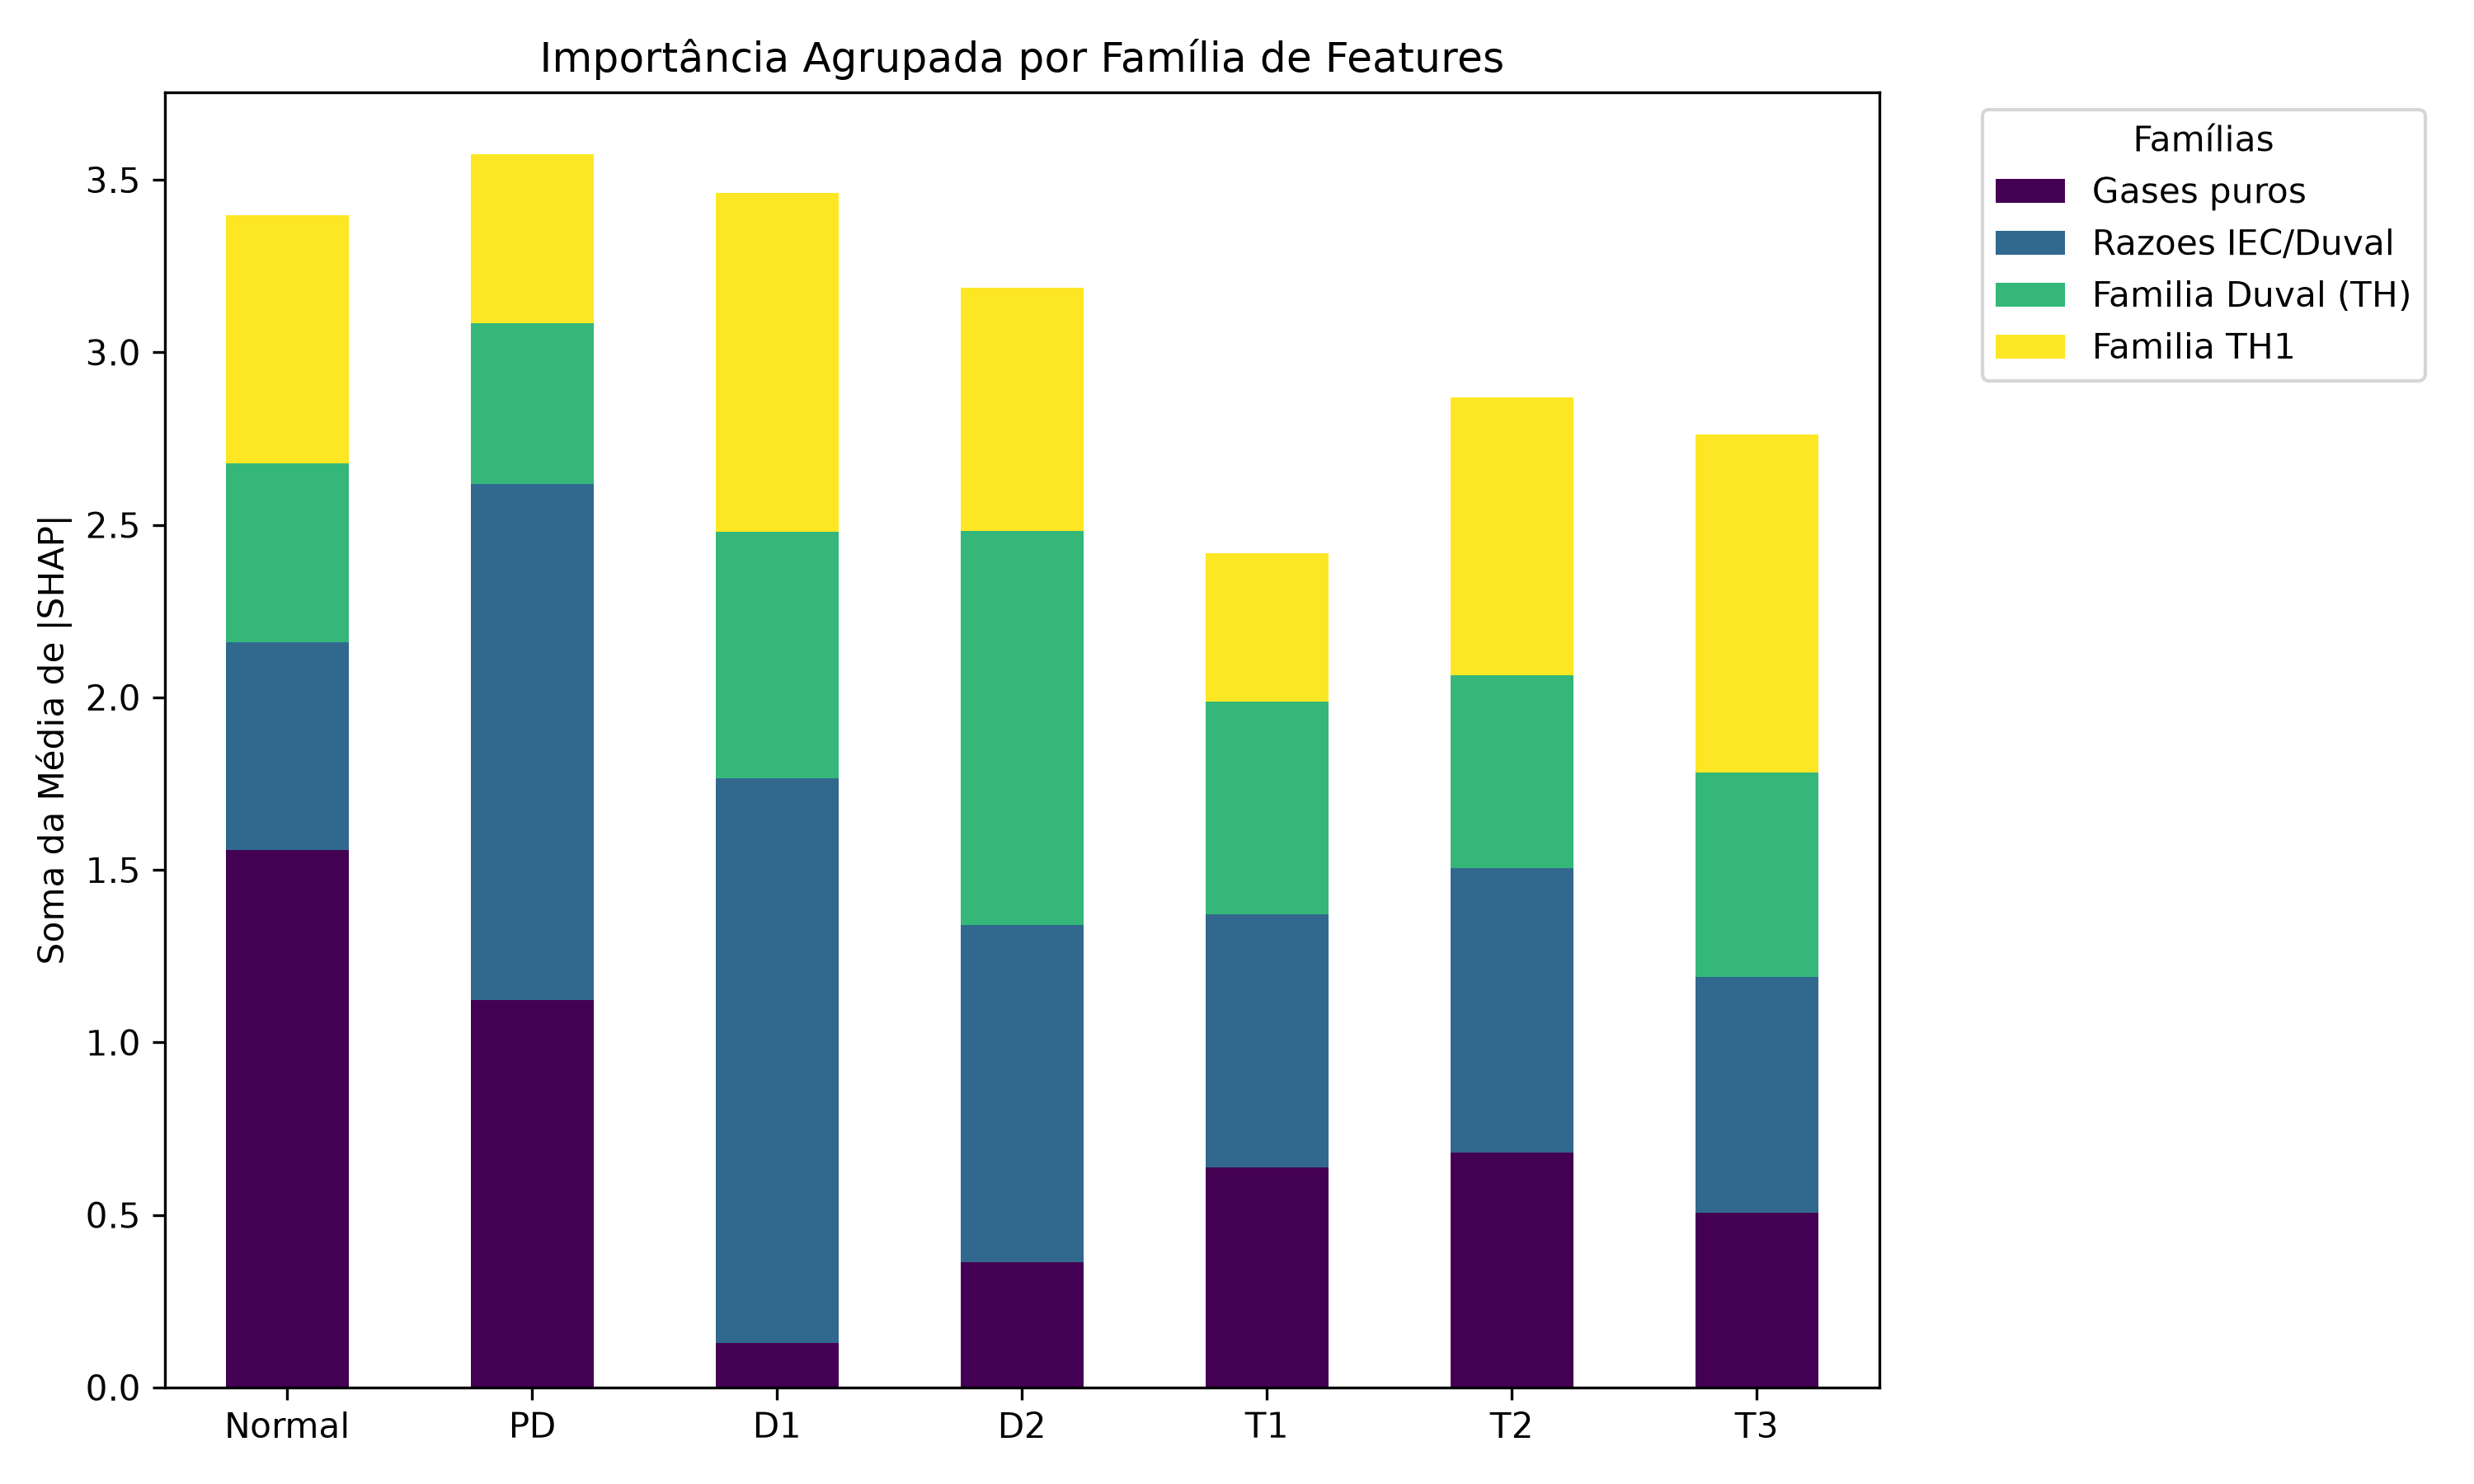
\includegraphics[width=0.85\textwidth]{figuras/fase6/fig2_grouped_track_b.png}
\caption{Importância agregada por famílias de gases para as sete categorias de integridade operacional.}
\label{fig:shap_grouped}
\fonte{Elaborado pelo autor.}
\end{figure}

As descargas elétricas no óleo (D1 e D2) dependem prioritariamente das variáveis da família do acetileno, em especial das razões $\text{C}_2\text{H}_2/\text{TH}$ e $\text{C}_2\text{H}_2/\text{C}_2\text{H}_4$. Em contraste, as descargas parciais (PD) concentram a importância na família do metano e na razão $\text{CH}_4/\text{H}_2$, condizente com a geração de hidrogênio e metano sob descargas elétricas incipientes de baixa energia. Por sua vez, as falhas térmicas (T1, T2 e T3) dividem a importância entre os derivados de etileno ($\text{C}_2\text{H}_4/\text{TH}$) e etano ($\text{C}_2\text{H}_4/\text{C}_2\text{H}_6$), refletindo o aumento térmico que intensifica a formação de etileno.

\begin{figure}[htbp]
\centering
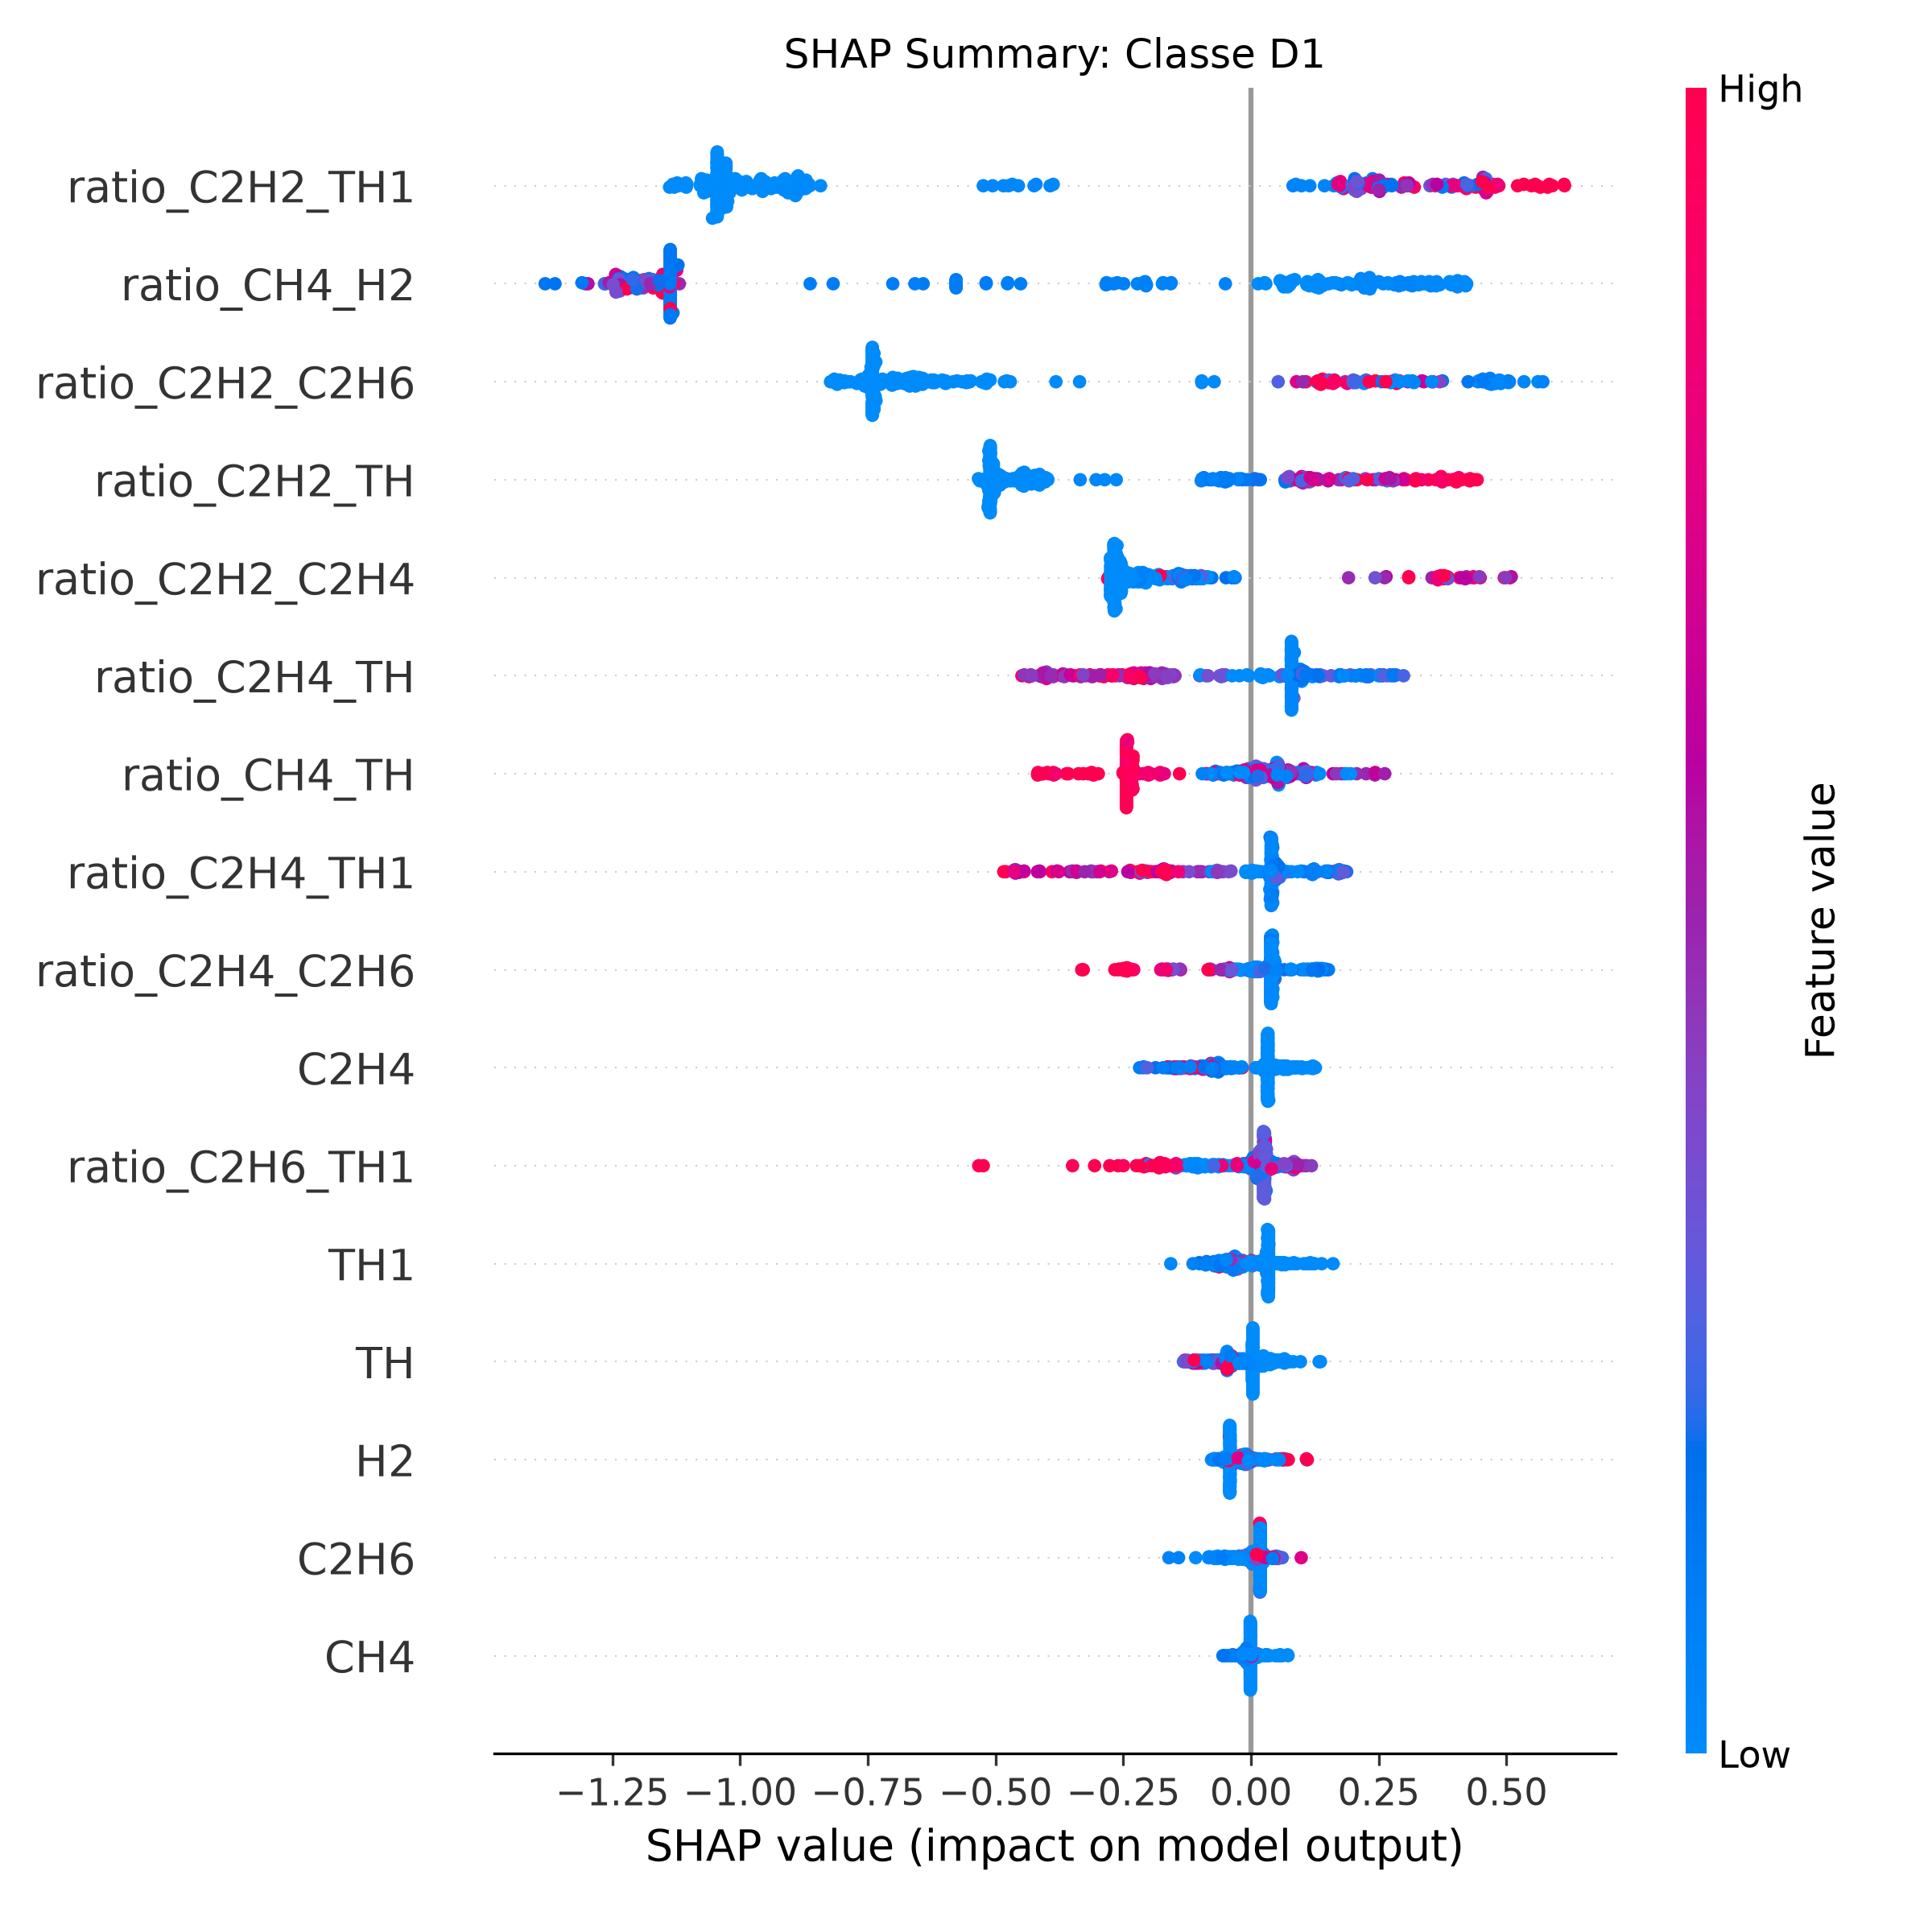
\includegraphics[width=0.85\textwidth]{figuras/fase6/fig3_beeswarm_D1.png}
\caption{Distribuição dos valores de SHAP para a classe de Descargas de Baixa Energia (D1).}
\label{fig:beeswarm_d1}
\fonte{Elaborado pelo autor.}
\end{figure}

O gráfico de dispersão (\textit{beeswarm}) para a classe D1 (Figura~\ref{fig:beeswarm_d1}) detalha esse comportamento em nível de amostra individual. Valores altos de $\text{C}_2\text{H}_2/\text{TH}$ e da razão $\text{C}_2\text{H}_2/\text{C}_2\text{H}_4$ deslocam a previsão fortemente na direção positiva da classe D1, enquanto proporções baixas ou nulas de acetileno reduzem a probabilidade dessa falha, confirmando o papel do acetileno como principal indicador de descargas elétricas.

\subsection{Extração de Limiares Físicos Marginais}

Utilizando a matriz de interações (\texttt{pred\_interactions}), isolou-se o efeito principal univariado ($\phi_{i,i}$) de cada variável diagnóstica na escala física original. O ponto em que a curva cruza a linha de contribuição nula ($\phi_{i,i} = 0$) identifica o limiar a partir do qual a variável passa a atuar a favor da ocorrência daquela falha. A Tabela~\ref{tab:limiares_fisicos} compara esses pontos de transição aprendidos pelo XGBoost com os limites fixados pelo Triângulo 1 de Duval e pela norma IEC 60599.

\begin{table}[htbp]
\centering
\caption{Comparação entre limiares analíticos normativos e pontos de transição marginal do TreeSHAP.}
\label{tab:limiares_fisicos}
\resizebox{\textwidth}{!}{%
\begin{tabular}{lccc}
\hline
\textbf{Parâmetro Químico} & \textbf{Falha Alvo} & \textbf{Limiar Normativo} & \textbf{Limiar Marginal Extraído} \\ \hline
Percentual $\% \text{C}_2\text{H}_4$ ($\text{C}_2\text{H}_4/\text{TH}$) & D1 & $< 23\%$ (Duval) & Faixa entre 20\% e 25\% \\
Percentual $\% \text{C}_2\text{H}_2$ ($\text{C}_2\text{H}_2/\text{TH}$) & D1 & $\ge 13\%$ (Duval) & $\approx 8,0\%$ \\
Percentual $\% \text{C}_2\text{H}_2$ ($\text{C}_2\text{H}_2/\text{TH}$) & D2 & $\ge 13\%$ ou $29\%$ (Duval) & $\approx 8,6\%$ \\
Razão $\text{C}_2\text{H}_4/\text{C}_2\text{H}_6$ & T3 & $> 4,0$ (IEC 60599) & $\approx 2,97$ \\ \hline
\end{tabular}%
}
\fonte{Elaborado pelo autor.}
\end{table}

\begin{figure}[htbp]
\centering
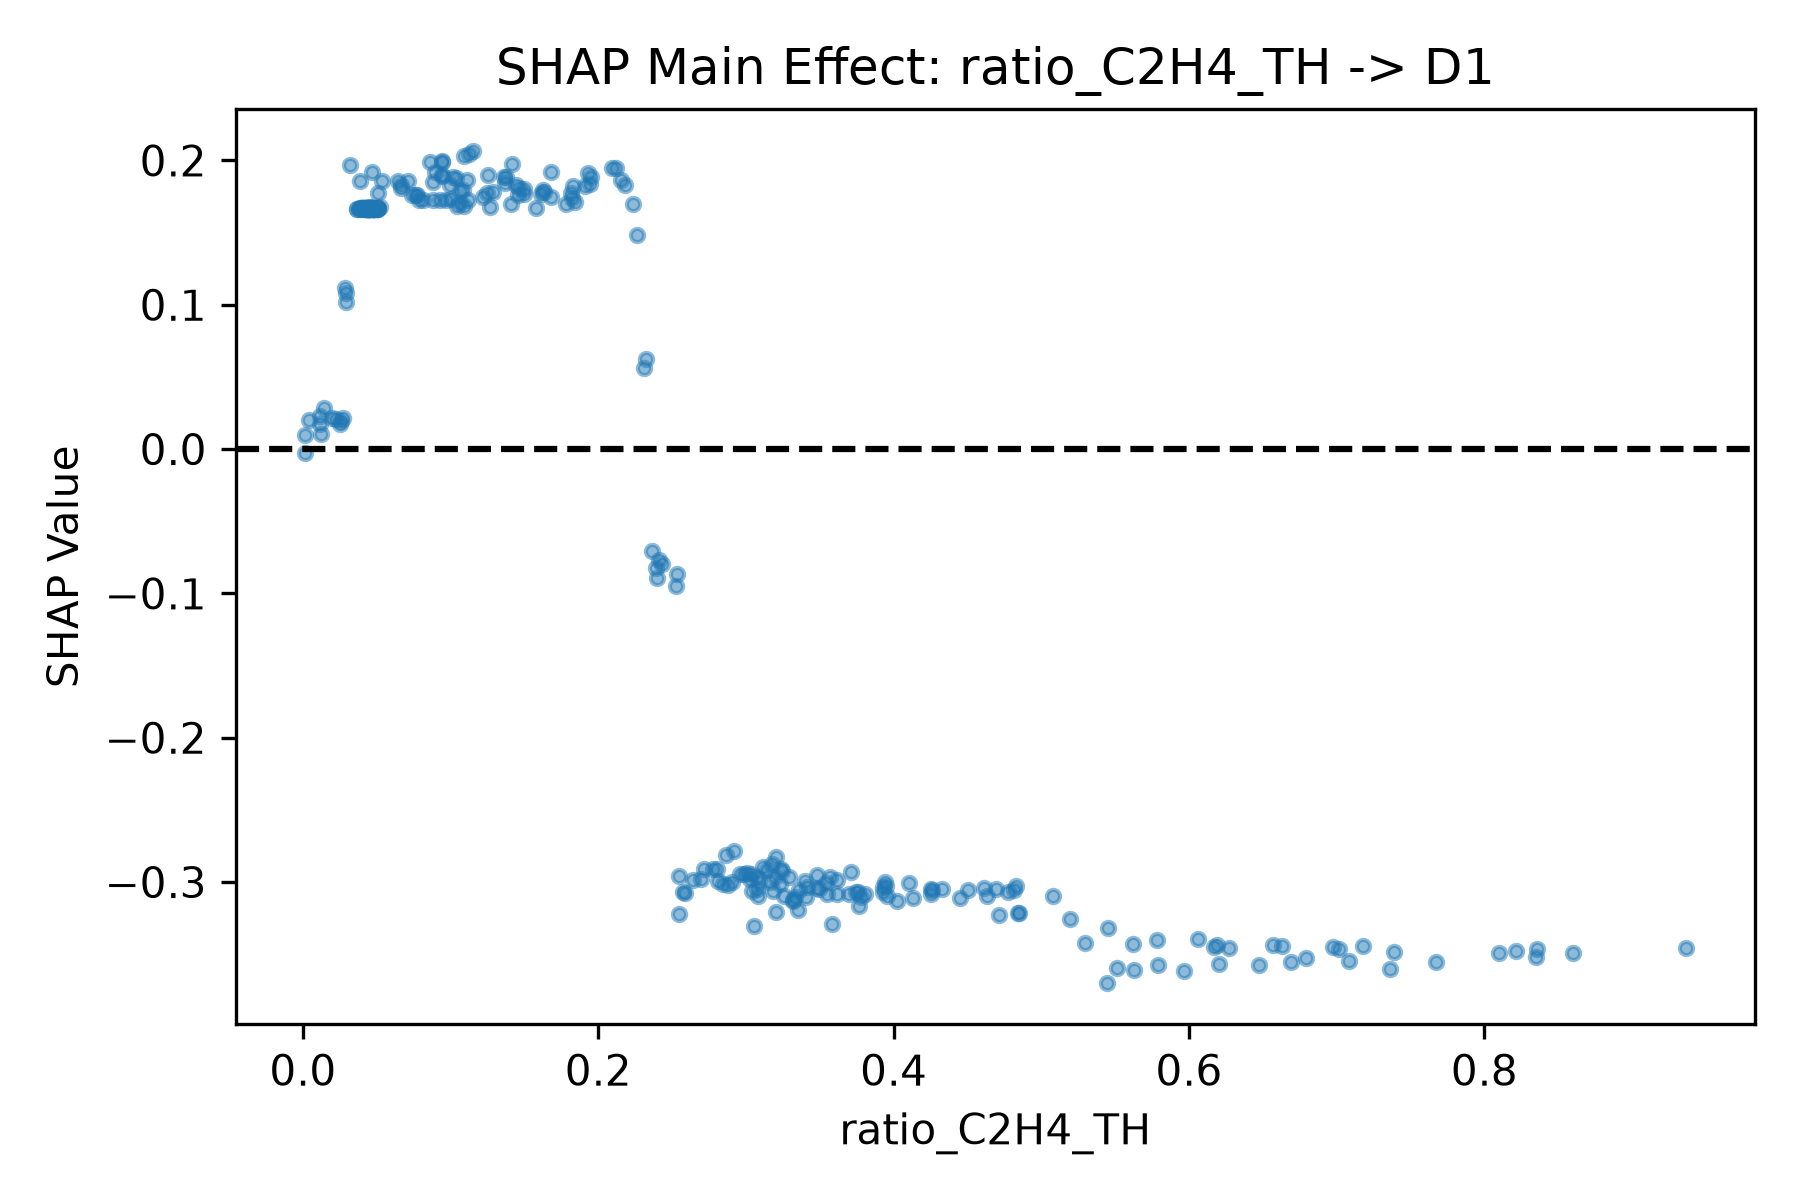
\includegraphics[width=0.85\textwidth]{figuras/fase6/fig4_thresh_ratio_C2H4_TH_D1.png}
\caption{Efeito principal isolado do TreeSHAP para a razão $\text{C}_2\text{H}_4/\text{TH}$ na classe D1.}
\label{fig:shap_thresh_c2h4}
\fonte{Elaborado pelo autor.}
\end{figure}

Conforme ilustrado na Figura~\ref{fig:shap_thresh_c2h4}, o efeito principal da razão $\text{C}_2\text{H}_4/\text{TH}$ na identificação de D1 cruza a linha neutra $\phi_{i,i} = 0$ na faixa entre 0,20 e 0,25 (20\% a 25\%), valor condizente com o limite de 23\% fixado pelo Triângulo 1 de Duval para separar descargas de baixa energia de falhas com componente térmico.

Por outro lado, o limiar aprendido para a porcentagem de acetileno em D1 e D2 situou-se em torno de 8\%, valor mais sensível que o corte normativo tradicional de 13\%. Esse comportamento decorre da base de dados, na qual transformadores com laudo de descarga elétrica já apresentavam diagnóstico mesmo com teores menores de $\text{C}_2\text{H}_2$. De modo semelhante, o limiar da razão $\text{C}_2\text{H}_4/\text{C}_2\text{H}_6$ para T3 fixou-se em 2,97, condizente com a característica das amostras de T3 da base mencionada anteriormente. Para os casos de T3 com menor proporção de etileno, o modelo apoia-se complementarmente no percentual de etano sobre os hidrocarbonetos totais (\texttt{ratio\_C2H6\_TH1}), conforme indicado no mapa de calor da Figura~\ref{fig:shap_heatmap}. Vale notar que o ponto $\phi_{i,i} = 0$ indica o momento em que a variável passa a exercer contribuição positiva, não se tratando de uma barreira rígida e isolada.

\subsection{Visualização Espacial no Triângulo de Duval}

Para visualizar o comportamento do classificador no espaço geométrico tradicional, as 295 amostras do conjunto de teste foram projetadas sobre as coordenadas do Triângulo 1 de Duval ($\% \text{CH}_4$, $\% \text{C}_2\text{H}_4$ e $\% \text{C}_2\text{H}_2$). A Figura~\ref{fig:duval_erros} apresenta essa projeção, destacando a localização dos acertos e dos erros diagnósticos.

\begin{figure}[htbp]
\centering
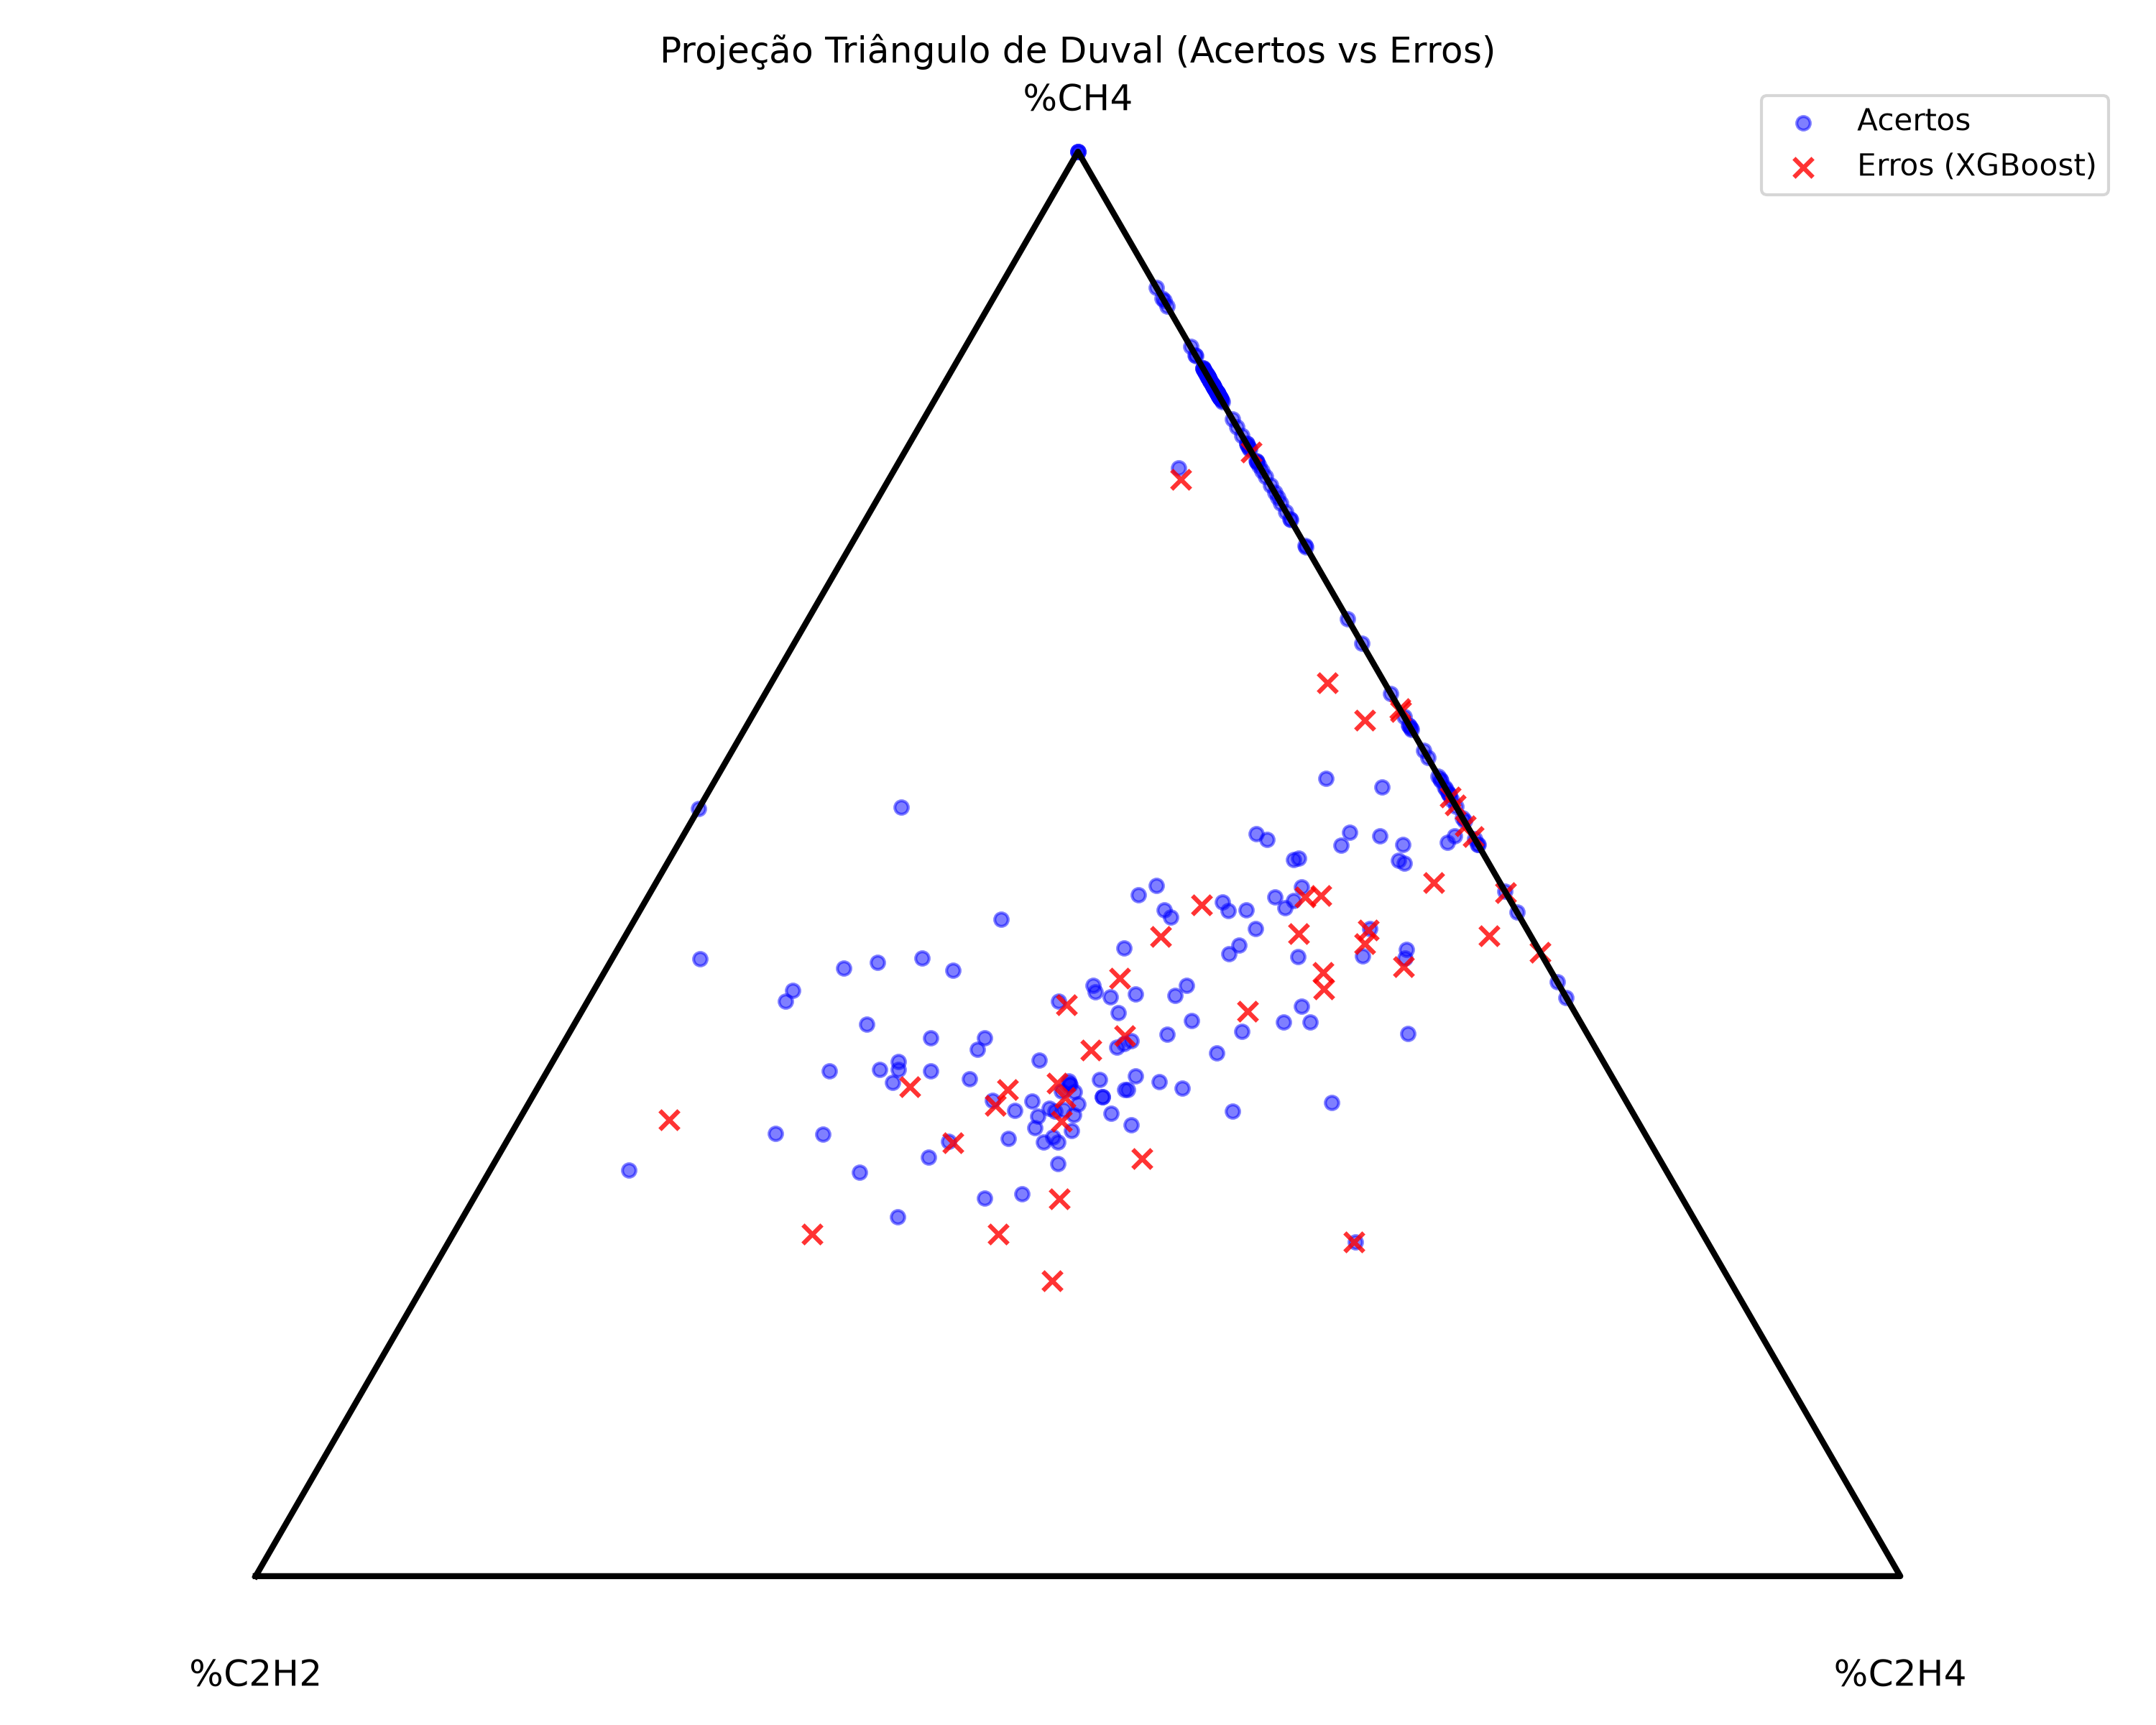
\includegraphics[width=0.85\textwidth]{figuras/fase6/fig5_duval_triangle.png}
\caption{Mapeamento das amostras de teste no Triângulo 1 de Duval com a localização dos erros diagnósticos.}
\label{fig:duval_erros}
\fonte{Elaborado pelo autor.}
\end{figure}

A visualização indica que os erros do XGBoost concentram-se nas imediações das fronteiras que separam as zonas D1 e D2 ou na zona de transição DT (térmica e elétrica combinadas), faixas em que a própria norma reconhece sobreposição e incerteza física de diagnóstico.

\subsection{Análise Local de Erros de Classificação}

A decomposição aditiva local por gráficos em cascata (\textit{waterfall plots}) permite examinar em detalhe os fatores que levaram o modelo a uma determinada previsão. A Figura~\ref{fig:waterfall_d1_d2} apresenta essa análise para a amostra de índice 11 do conjunto de teste, cujo diagnóstico original de campo era D1, mas que foi classificada pelo modelo como D2.

\begin{figure}[htbp]
\centering
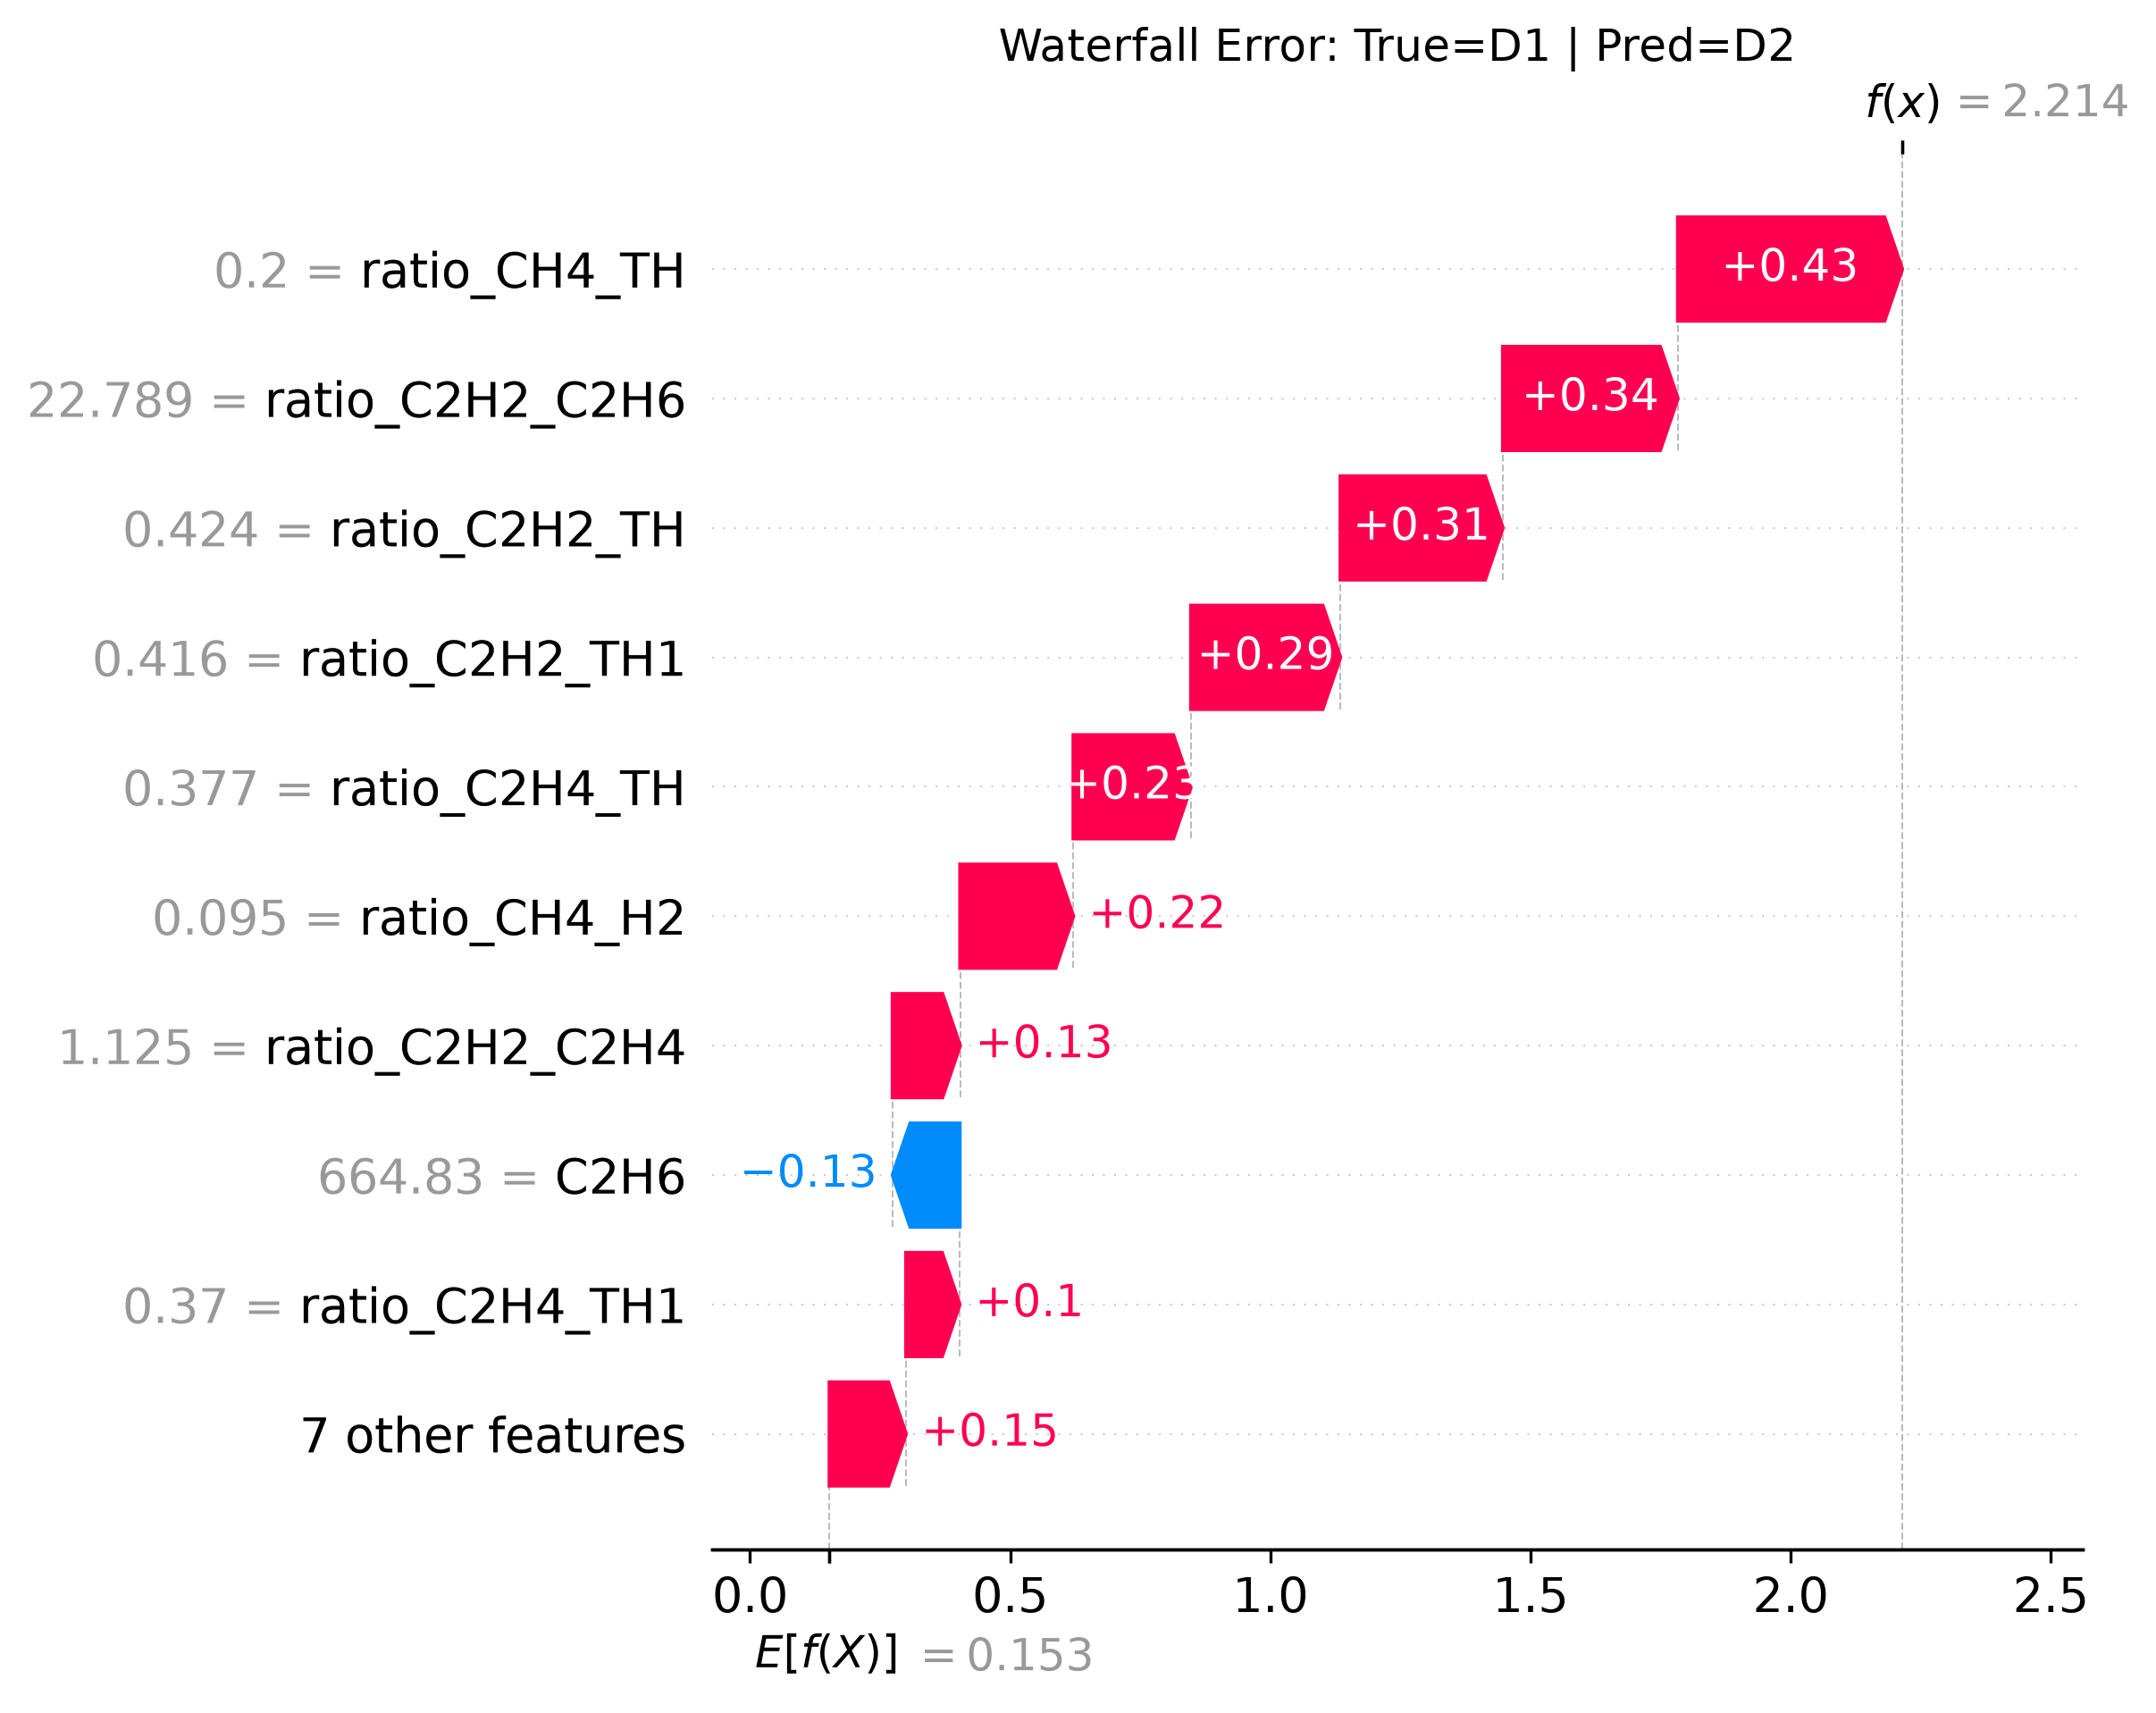
\includegraphics[width=0.85\textwidth]{figuras/fase6/fig6_waterfall_error_D1_to_D2_11.png}
\caption{Decomposição aditiva via Waterfall plot de um caso classificado de D1 para D2 (amostra 11).}
\label{fig:waterfall_d1_d2}
\fonte{Elaborado pelo autor.}
\end{figure}

O gráfico da Figura~\ref{fig:waterfall_d1_d2} mostra a evolução a partir do valor basal $\mathbb{E}[f(X)] = 0,153$ até a margem final de predição $f(x) = 2,214$ em favor da classe D2. Observa-se que a proporção de etileno (\texttt{ratio\_C2H4\_TH}) foi de 0,377 (37,7\%), exercendo um impacto positivo de $+0,23$ para a classificação em D2, o que é coerente com a regra do Triângulo de Duval em que teores de etileno acima de 23\% saem da faixa de descargas de baixa energia D1. Além disso, a presença expressiva de acetileno gerou contribuições positivas adicionais para D2 ($+0,34$ em \texttt{ratio\_C2H2\_C2H6}, $+0,31$ em \texttt{ratio\_C2H2\_TH} e $+0,29$ em \texttt{ratio\_C2H2\_TH1}). A concentração de etano ($\text{C}_2\text{H}_6 = 664,83$~ppm) exerceu leve papel redutor ($-0,13$), mas insuficiente para conter a tendência geral. Essa análise exemplifica como o modelo pondera a combinação de múltiplos gases em amostras limítrofes entre duas classes vizinhas.

\subsection{Migração de Crédito e Avaliação da Hipótese Temporal}

Para concluir a investigação sobre o papel das previsões da LSTM no Track A, avaliou-se como a importância atribuída pelo TreeSHAP se distribui entre variáveis medidas e variáveis previstas. A Figura~\ref{fig:migracao_credito} ilustra a importância média do hidrogênio dividida entre a leitura atual ($\text{H}_{2,\text{obs}}$) e as projeções futuras para 14 e 28 passos ($\text{H}_{2,\text{h14}}$ e $\text{H}_{2,\text{h28}}$).

\begin{figure}[htbp]
\centering
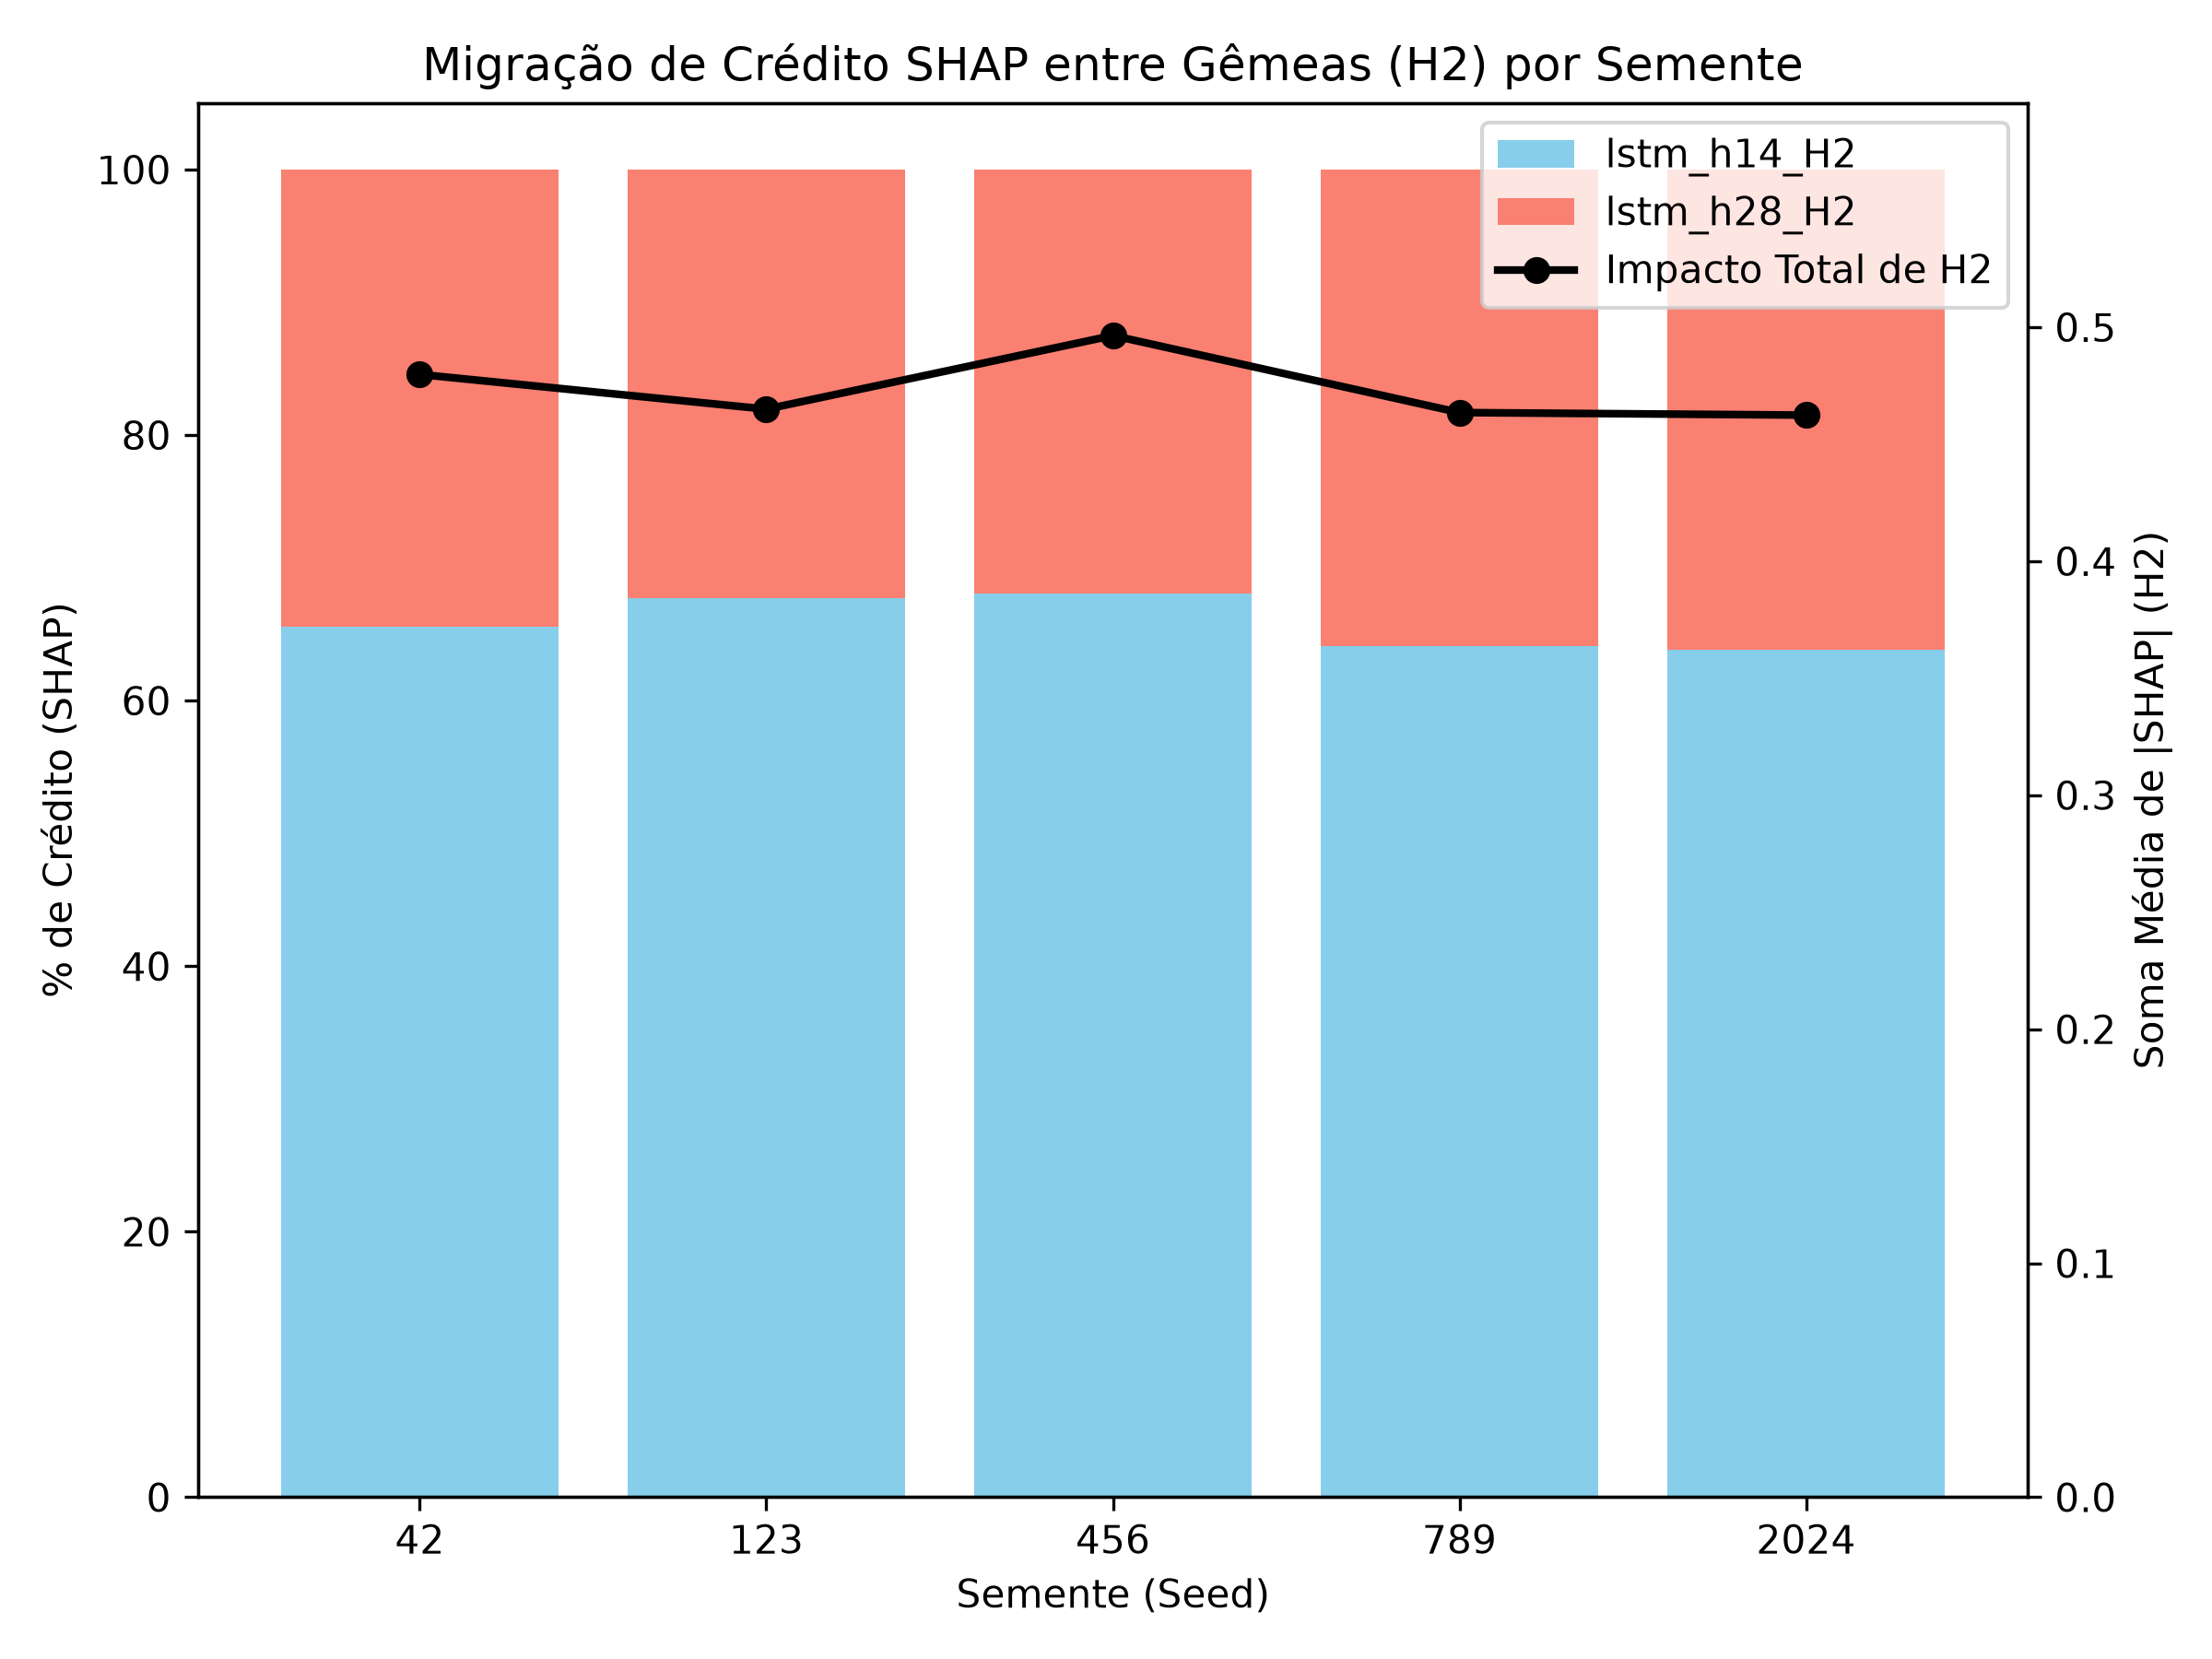
\includegraphics[width=0.85\textwidth]{figuras/fase6/fig7_lstm_credit_migration.png}
\caption{Divisão da importância do SHAP entre concentrações observadas e previstas pela LSTM.}
\label{fig:migracao_credito}
\fonte{Elaborado pelo autor.}
\end{figure}

O comportamento observado na Figura~\ref{fig:migracao_credito} esclarece por que a inclusão das previsões da LSTM não trouxe ganho estatístico no Track A. Quando se varia a semente de treinamento do XGBoost, a importância individual oscila entre a leitura do momento e as previsões futuras ($\text{H}_{2,\text{h14}}$ e $\text{H}_{2,\text{h28}}$), comportamento comum em árvores de decisão quando há variáveis fortemente correlacionadas. No entanto, a soma total da importância da família do hidrogênio (linha escura) permanece estável e praticamente idêntica à importância que o hidrogênio observado já recebia sozinho no modelo puramente estático. Isso confirma que as projeções futuras da rede neural não trazem informação independente nova para a decisão pontual, explicando por que a combinação temporal não superou o classificador baseado apenas nas leituras do momento.
